\documentclass[notes,10pt, aspectratio=169]{beamer}

\usepackage{pgfpages}
% These slides also contain speaker notes. You can print just the slides,
% just the notes, or both, depending on the setting below. Comment out the want
% you want.
\setbeameroption{hide notes} % Only slide
%\setbeameroption{show only notes} % Only notes
%\setbeameroption{show notes on second screen=right} % Both
\usepackage{wrapfig}

\usepackage{helvet}
\usepackage[default]{lato}
\usepackage{array}
\usepackage{eurosym}
\usepackage{setspace}
\usepackage{animate}
\usepackage{multicol}
\usepackage{breqn}
\usepackage{subcaption}
\usepackage{caption}
\captionsetup{font=scriptsize, justification=raggedright,singlelinecheck=false}
\usepackage[export]{adjustbox}
\usepackage[scale=2]{ccicons}
\usepackage{tikz}
\newenvironment{wideitemize}{\itemize\addtolength{\itemsep}{10pt}}{\enditemize}
\usepackage{natbib}

\usepackage{tikz}
\usepackage{verbatim}
\setbeamertemplate{note page}{\pagecolor{yellow!5}\insertnote}
\usepackage{amsmath}
%\usepackage{mathpazo}
\usepackage{hyperref}
\usepackage{lipsum}
\usepackage{multimedia}
\usepackage{multirow}
\usepackage{graphicx}
\usepackage{dcolumn}
\usepackage{bbm}
\newcolumntype{d}[0]{D{.}{.}{5}}

\usepackage{changepage}
\usepackage{appendixnumberbeamer}
% \newcommand{\beginbackup}{
%   \newcounter{framenumbervorappendix}
%   \setcounter{framenumbervorappendix}{\value{framenumber}}
%   \setbeamertemplate{footline}
%   {
%      \leavevmode%
%      \hline
%      box{%
%       \begin{beamercolorbox}[wd=\paperwidth,ht=2.25ex,dp=1ex,right]{footlinecolor}%
% %         \insertframenumber  \hspace*{2ex} 
%       \end{beamercolorbox}}%
%      \vskip0pt%
%   }
%  }
\useinnertheme[shadow]{rounded}
\setbeamercolor{block title example}{fg=black,bg=orange!50!white}
\setbeamercolor{block body example}{fg=black, bg=orange!30!white}
\setbeamercolor{block title}{use=structure,fg=structure.fg,bg=structure.fg!20!bg}
\setbeamercolor{block body}{parent=normal text,use=block title,bg=block title.bg!50!bg}

 \setbeamertemplate{footline}{
    \hbox{%
    \begin{beamercolorbox}[wd=\paperwidth,ht=3ex,dp=1.5ex,leftskip=2ex,rightskip=2ex]{page footer}%
        %\usebeamerfont{title in head/foot}%
        %\insertshorttitle \hfill
        %\insertsection \hfill
        %\tableofcontents[currentsection] \hfill
        \insertsectionnavigationhorizontal{0.7\paperwidth}{}{} \hfill 
        \insertframenumber{} / \inserttotalframenumber
    \end{beamercolorbox}}%
}
\newcommand{\backupend}{
   \addtocounter{framenumbervorappendix}{-\value{framenumber}}
   \addtocounter{framenumber}{\value{framenumbervorappendix}} 
}


\usepackage{graphicx}
\usepackage[space]{grffile}
\usepackage{booktabs}

% These are my colors -- there are many like them, but these ones are mine.
\definecolor{blue}{RGB}{0,114,178}
\definecolor{red}{RGB}{213,94,0}
\definecolor{yellow}{RGB}{240,228,66}
\definecolor{green}{RGB}{0,158,115}

\setbeamercolor{section in head/foot}{fg=blue}


\hypersetup{
  colorlinks=false,
  linkbordercolor = {white},
  linkcolor = {blue}
}


%% I use a beige off white for my background
\definecolor{MyBackground}{RGB}{255,253,218}

%% Uncomment this if you want to change the background color to something else
%\setbeamercolor{background canvas}{bg=MyBackground}

%% Change the bg color to adjust your transition slide background color!
\newenvironment{transitionframe}{
  \setbeamercolor{background canvas}{bg=yellow}
  \begin{frame}}{
    \end{frame}
}

\setbeamercolor{frametitle}{fg=blue}
\setbeamercolor{title}{fg=black}
%\setbeamertemplate{footline}[frame number]
\setbeamertemplate{navigation symbols}{} 
\setbeamertemplate{itemize items}{-}
\setbeamercolor{itemize item}{fg=blue}
\setbeamercolor{itemize subitem}{fg=blue}
\setbeamercolor{enumerate item}{fg=blue}
\setbeamercolor{enumerate subitem}{fg=blue}
\setbeamercolor{button}{bg=white,fg=blue,}



% If you like road maps, rather than having clutter at the top, have a roadmap show up at the end of each section 
% (and after your introduction)
% Uncomment this is if you want the roadmap!
% \AtBeginSection[]
% {
%    \begin{frame}
%        \frametitle{Roadmap of Talk}
%        \tableofcontents[currentsection]
%    \end{frame}
% }
\setbeamercolor{section in toc}{fg=blue}
\setbeamercolor{subsection in toc}{fg=red}
%\setbeamersize{text margin left=1em,text margin right=1em} 
\setbeamersize{text margin left=0.7cm,text margin right=0.7cm} 


\title[]{\textcolor{blue}{Lecture 3 v2:\\Simple Linear Regression}}
\author{25117 - Econometrics}
\institute[shortinst]{Universitat Pompeu Fabra}

\date{October 7th, 2024}

\begin{document}



% Title Slide

\begin{frame}[plain]
\maketitle
\end{frame}

\section{Introduction}

\begin{frame}{What we learned in the last lesson}
\begin{itemize}
    \item The sample average, $\overline{Y}$, is an estimator of the population mean, $\mu_Y$. When $Y_1, \dots ,Y_n$ are i.i.d.,
    \begin{enumerate}
        \item  The sampling distribution of $\overline{Y}$ has mean $\mu_Y$ and variance $\sigma_{\overline{Y}}^2=\sigma_Y^2/n$
        \item $\overline{Y}$ is unbiased
        \item by the LLN, $\overline{Y}$ is consistent; and
        \item by the CLT, $\overline{Y}$ has an approximately normal sampling distribution when the $n$ is large.
    \end{enumerate}
    \item The t-statistic is used to test the null hypothesis that the population mean takes on a particular value. If $n$ is large, the t-stat $\sim \mathcal{N}(0,1)$ under $H_0$.
    \item The t-statistic can be used to calculate the p-value associated with the null hypothesis. The p-value is the probability of drawing a statistic at least as adverse to the null hypothesis as the one you actually computed in your sample, assuming the null hypothesis is correct. A small p-value is evidence that the null hypothesis is false.
    \item A 95\% confidence interval for $\mu_Y$ contains the true value of $\mu_Y$ in 95\% of all possible samples.
    \item The sample correlation coefficient is an estimator of the population correlation coefficient and measures the linear relationship between two variables -- that is, how well their scatterplot is approximated by a straight line.
\end{itemize}
\end{frame}


\begin{frame}{The regression line}
 \begin{columns}
\begin{column}{0.35\textwidth}
    \begin{itemize}
        \item The population regression line is the expected value of Y given X.
        \item The slope is the difference in the expected values of Y, for two values of X that differ by one unit
    \end{itemize}
\end{column}
\begin{column}{0.7\textwidth}
\begin{figure}
  \centering
         \vspace{-1mm}
        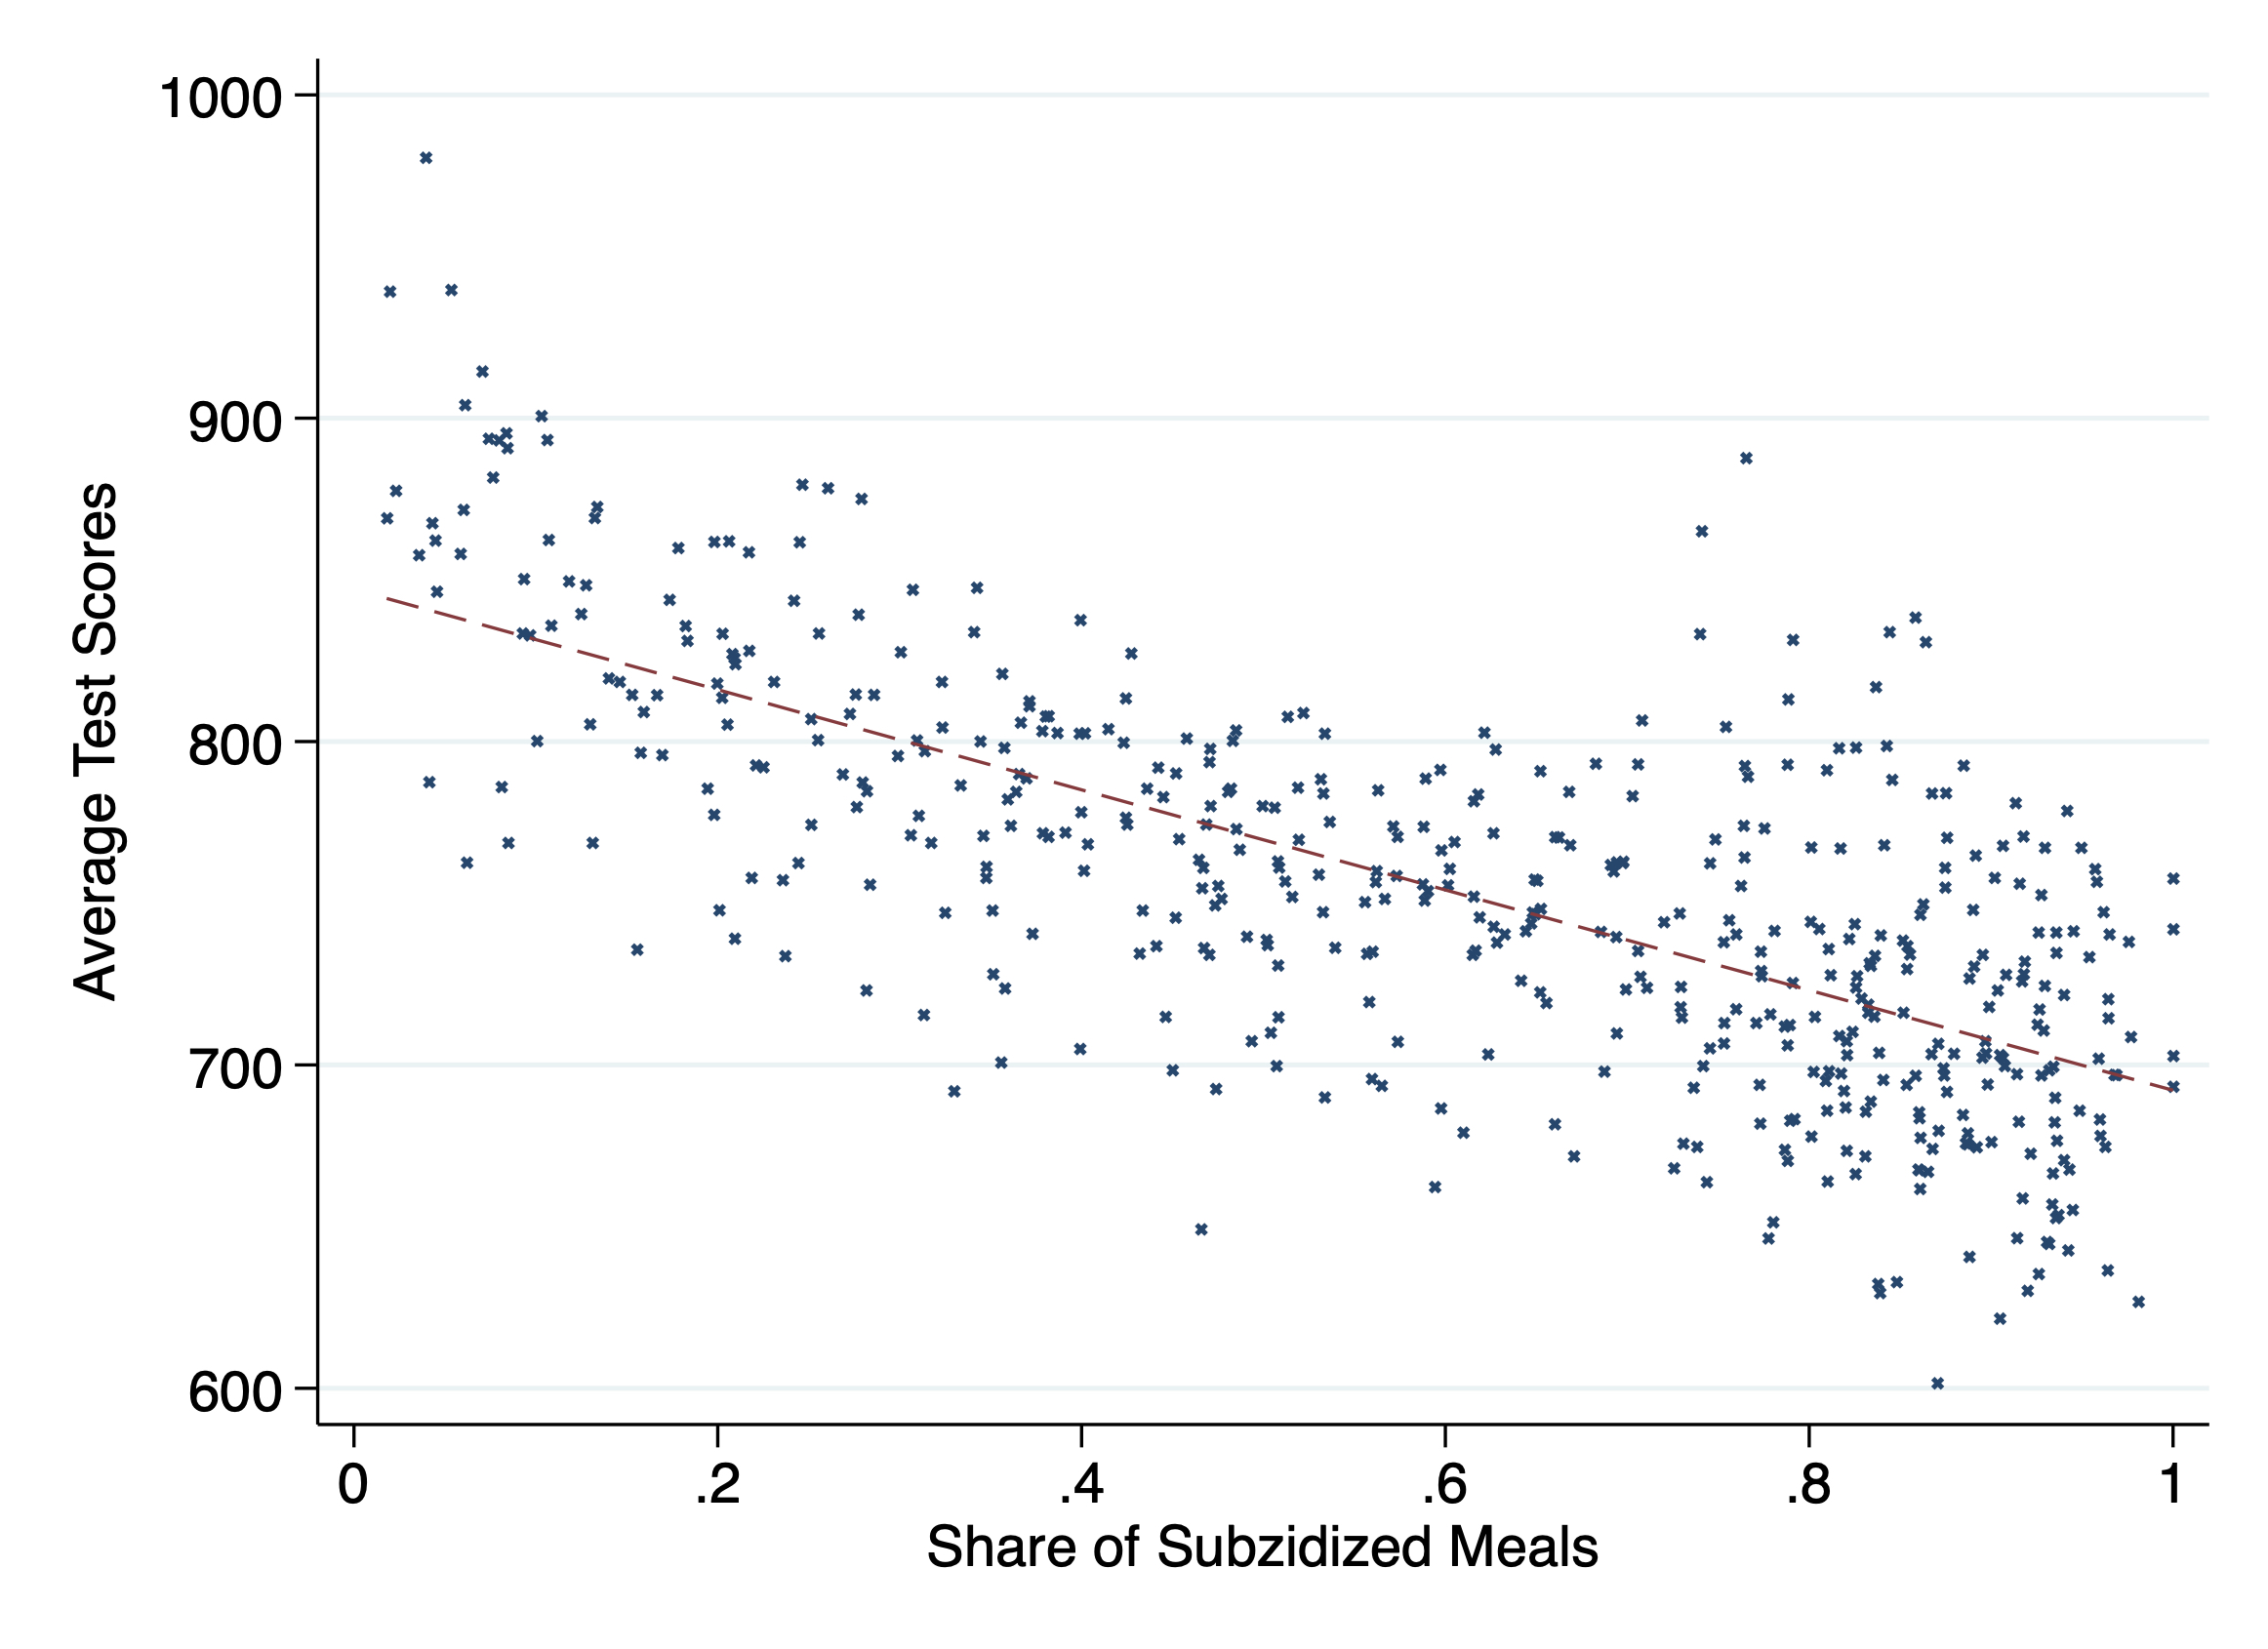
\includegraphics[scale=.25]{images/testscores_corr.png}
\end{figure}
\end{column}
\end{columns}
\end{frame}



\begin{frame}{The regression line}
 \begin{columns}
\begin{column}{0.35\textwidth}
 The estimated regression can be used either for
        \begin{enumerate}
            \item \textbf{causal inference} (learning about the causal effect on Y of a change in X)
            \begin{itemize}
                \item[$\rightarrow$] What is the causal impact of subsidizing meals on students' performances?
            \end{itemize}
            \item \textbf{prediction} (predicting the value of Y given X, for an observation not in the data set)
            \begin{itemize}
                \item[$\rightarrow$] What are the students' expected test scores given the share of subsidized meals?
            \end{itemize}
        \end{enumerate}
\end{column}
\begin{column}{0.7\textwidth}
\begin{figure}
  \centering
         \vspace{-1mm}
        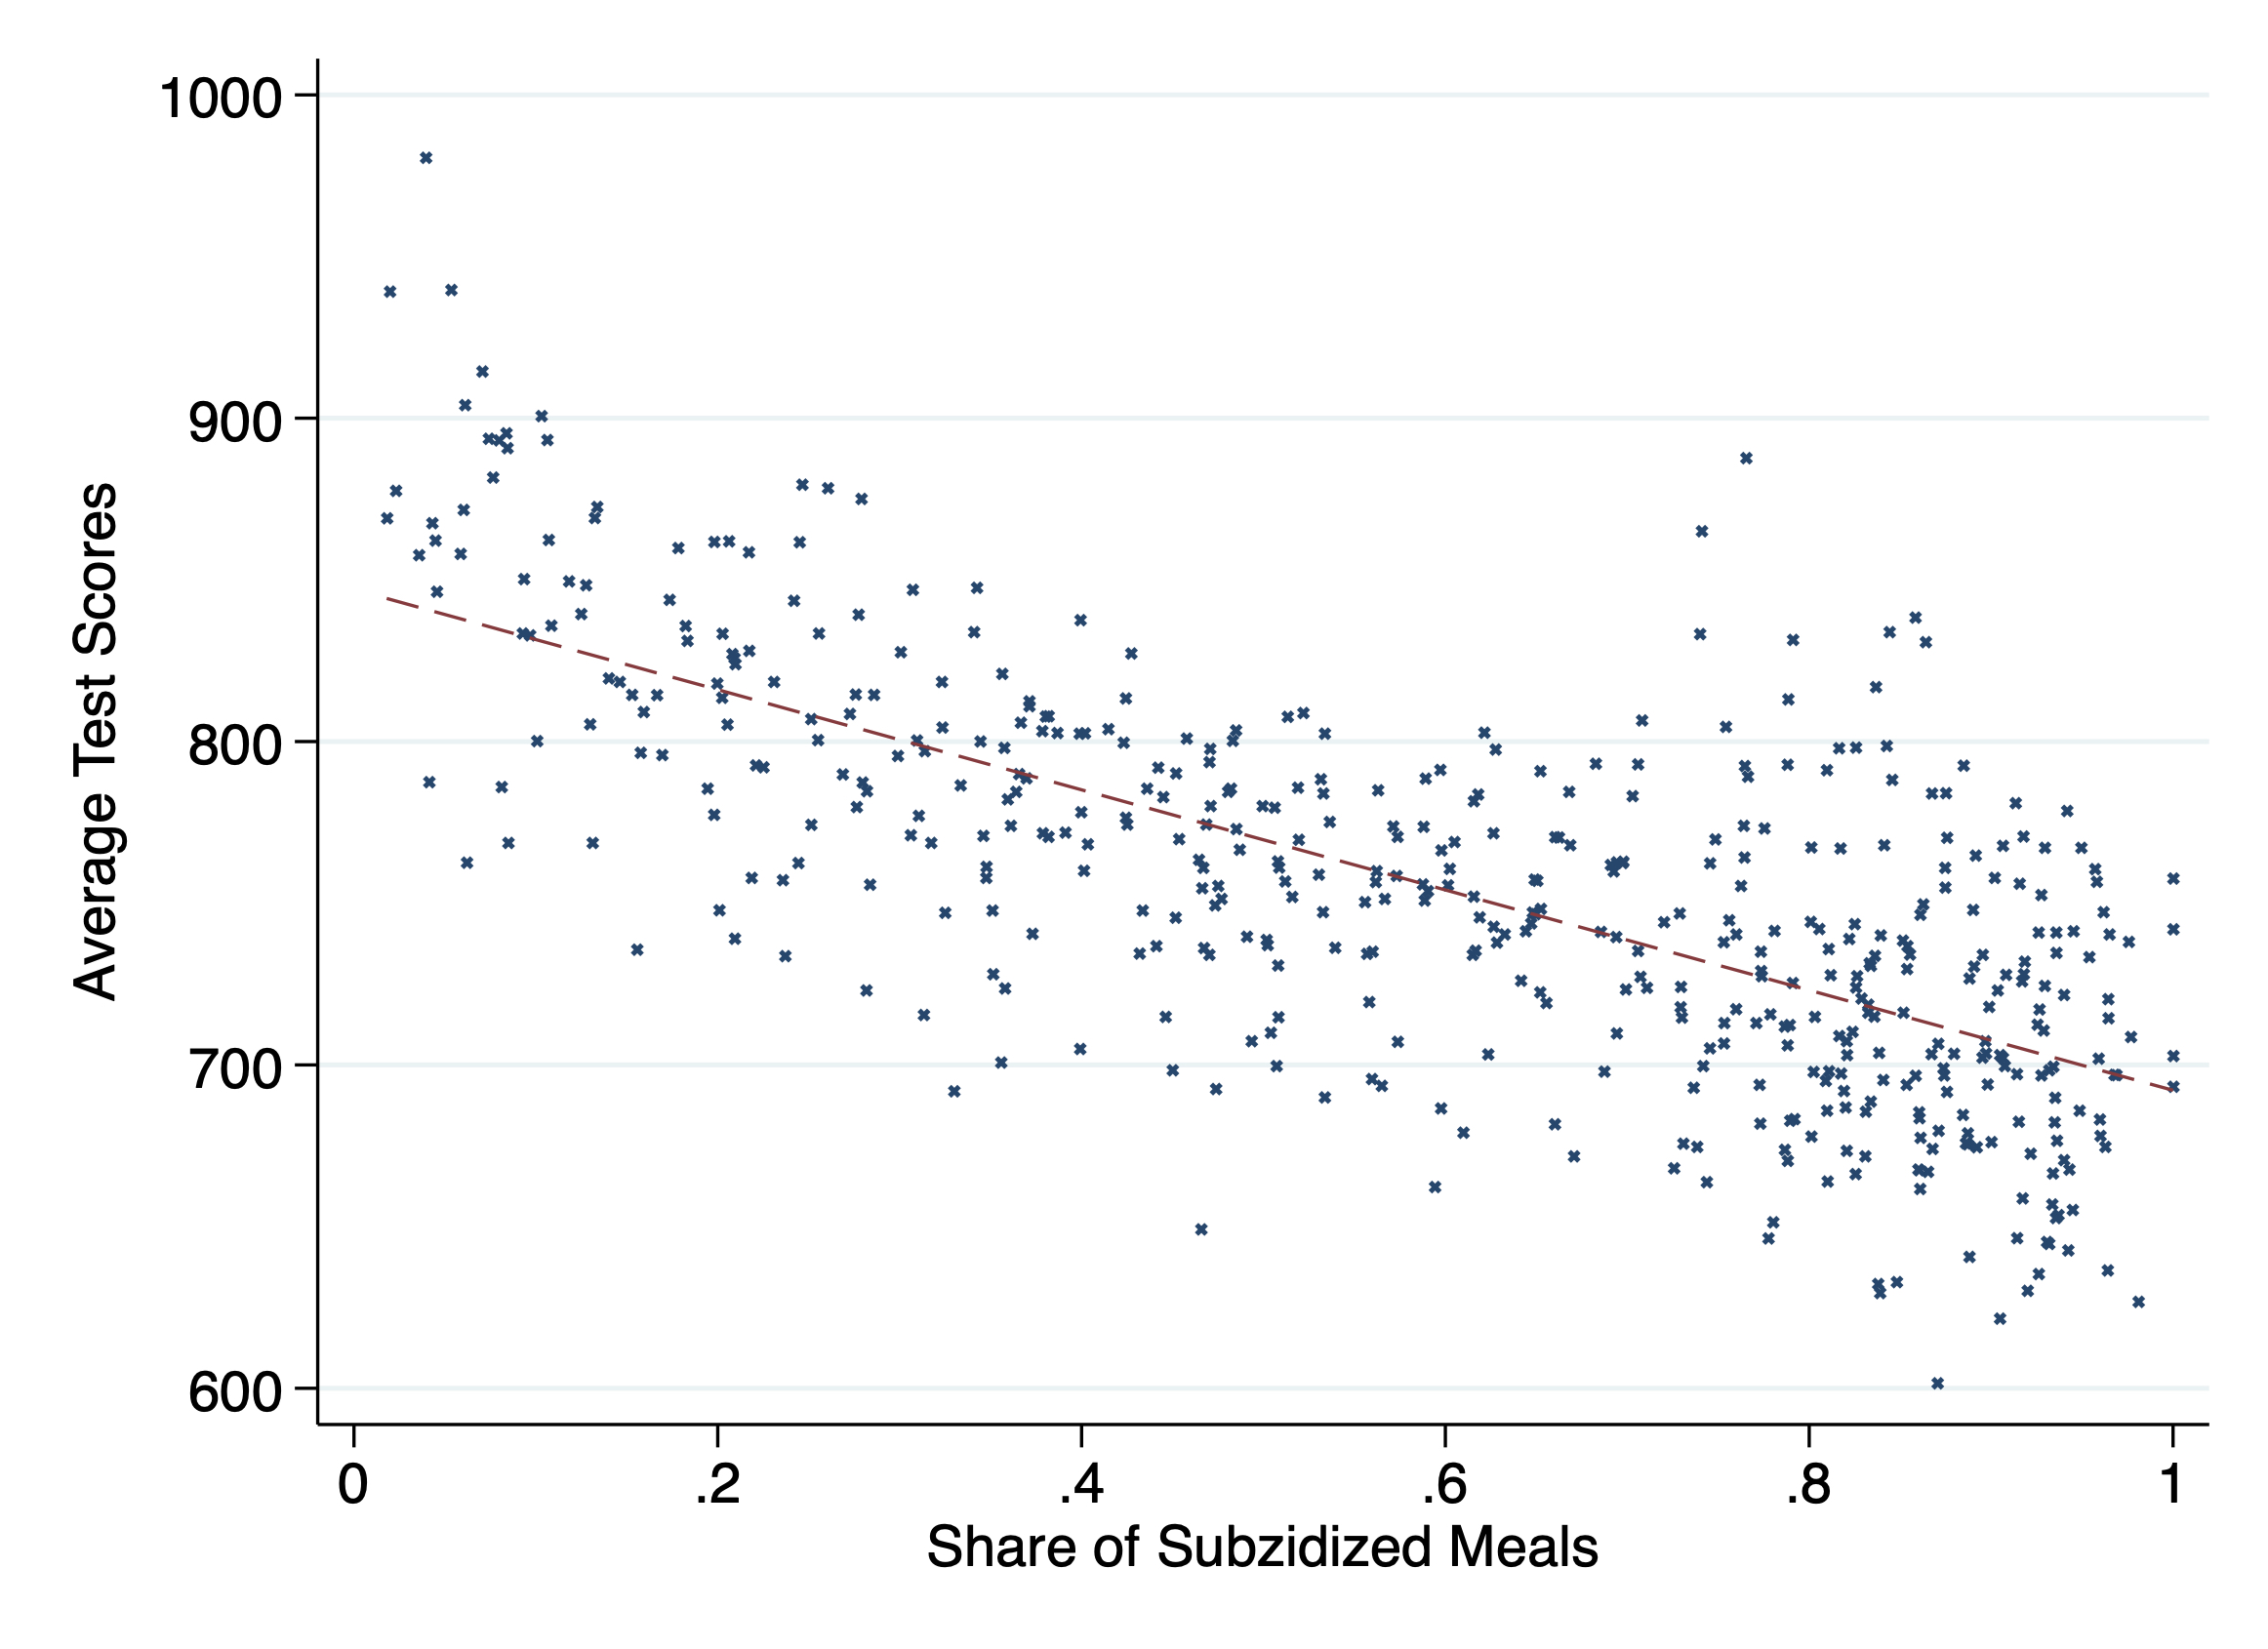
\includegraphics[scale=.25]{images/testscores_corr.png}
\end{figure}
\end{column}
\end{columns}
\end{frame}


\begin{frame}{The Population Linear Regression Model}
 \begin{columns}
\begin{column}{0.35\textwidth}
\begin{equation*}
    Y_i = \beta_0 + \beta_1 X_i + U_i
\end{equation*}
\begin{itemize}
    \item There are $n$ observations, $(X_i,Y_i)$, $i=\{1,\dots, n\}$
    \item $Y$ is the dependent variable
    \item $X$ is the independent variable or regressor
    \item $\mathbb{E}[Y\mid X] = \beta_0 + \beta_1 X$ is the population regression line
    \item $\beta_0$ is called the intercept
    \item $\beta_1$ is the slope
    \item $U_i$ is the random error; $u_i$ is its realization (as plotted).
\end{itemize}
\end{column}
\begin{column}{0.7\textwidth}
\begin{figure}
  \centering
         \vspace{-1mm}
        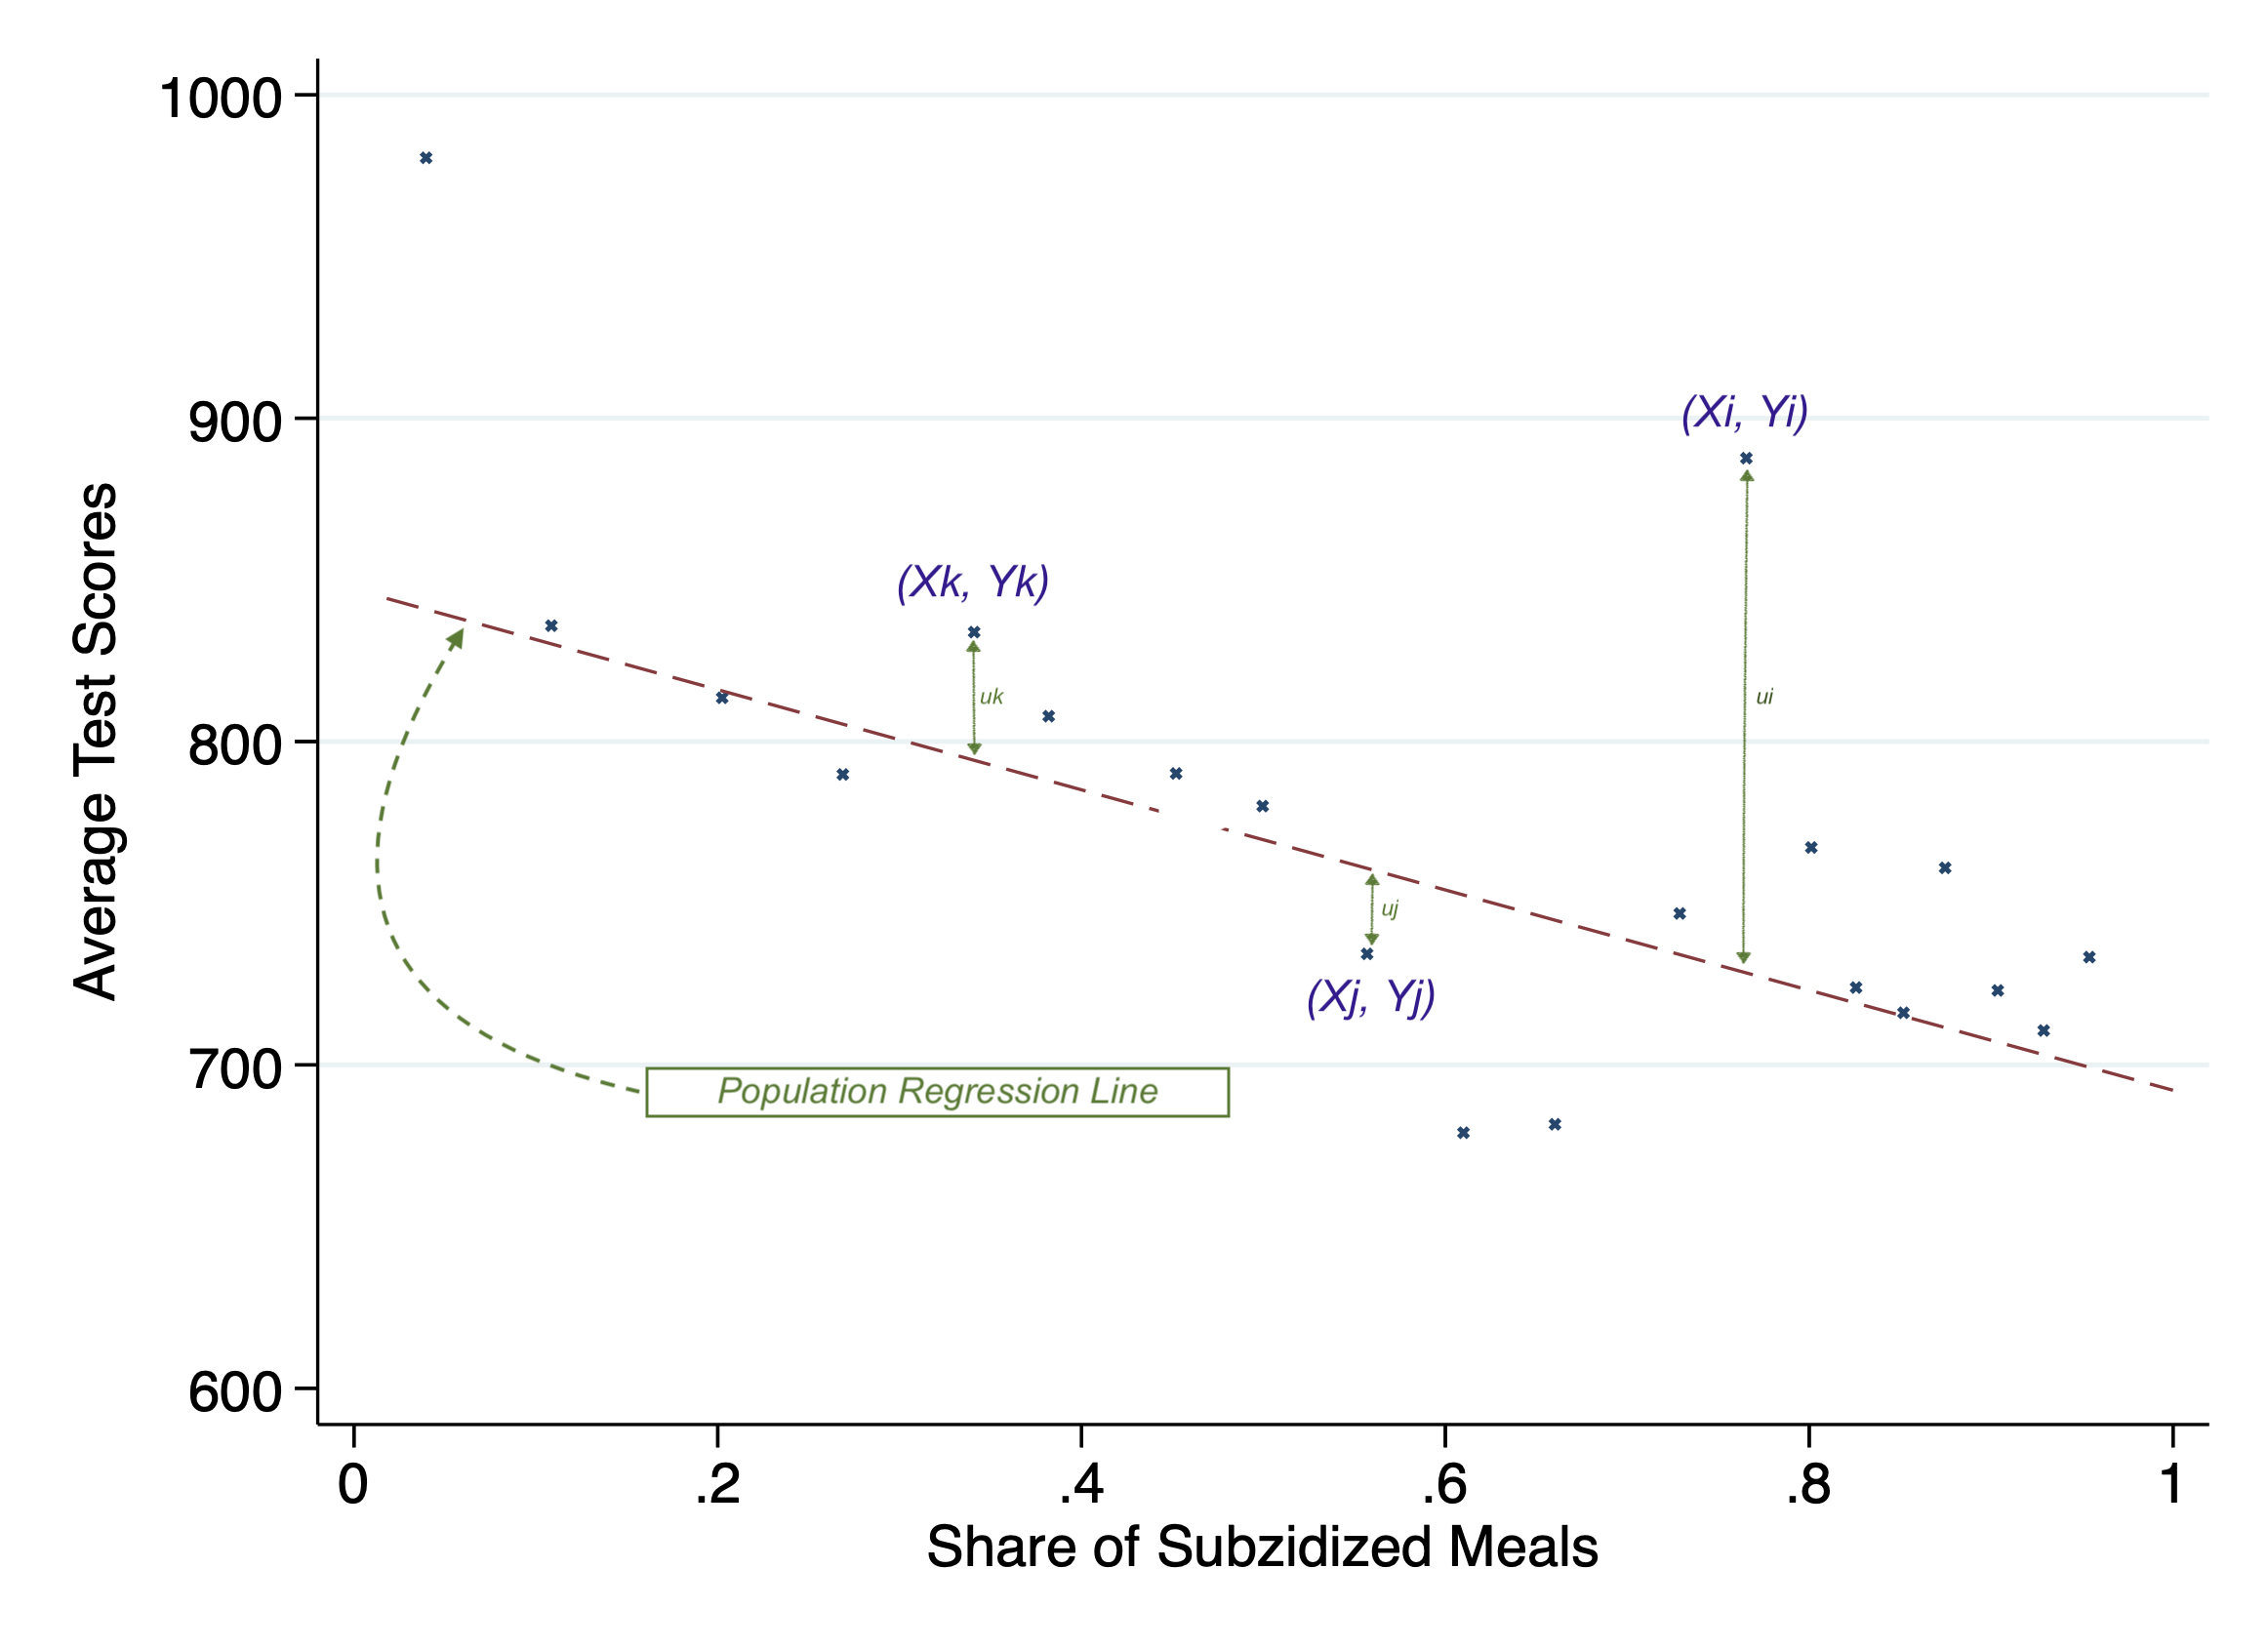
\includegraphics[scale=.25]{images/regression0.png}
\end{figure}
\end{column}
\end{columns}
\end{frame}



\begin{frame}{The Ordinary Least Squares (OLS) Estimator}
How can we estimate $\beta_0$ and $\beta_1$ from the data? Recall from Lecture 1 that the Least Square estimator of $\mu_Y$, $\overline{Y}$, solves
\begin{equation*}
    \min_m \sum_{i=1}^n (Y_i - m)^2
\end{equation*}
\\
By analogy, the OLS estimators of the unknown parameters $\beta_0$ and $\beta_1$,  $\hat{\beta}_0$ and $\hat{\beta}_1$ solves,
\begin{eqnarray*}
    &  &\min_{\beta_0, \beta_1} \sum_{i=1}^n U_i^2\\
    & \Leftrightarrow &\min_{\beta_0, \beta_1} \sum_{i=1}^n (Y_i - \mathbb{E}[Y\mid X])^2\\
   & \Leftrightarrow &\min_{\beta_0, \beta_1} \sum_{i=1}^n (Y_i - (\hat{\beta}_0 + \hat{\beta}_1 X_i))^2
\end{eqnarray*}
\end{frame}


\begin{frame}{The Ordinary Least Squares (OLS) Estimator}
\begin{itemize}
    \item The first-order conditions are
\end{itemize}
\begin{equation*}
\small
\sum_{i=1}^n\bigl(Y_i-\hat{\beta}_0-\hat{\beta}_1X_i\bigr)=0,
\qquad
\sum_{i=1}^n\bigl(Y_i-\hat{\beta}_0-\hat{\beta}_1X_i\bigr)X_i=0.
\end{equation*}
\begin{itemize}
    \item \textbf{Step 1: solve the first condition for the intercept.}
\end{itemize}
\begin{equation*}
\small
n\overline{Y}-n\hat{\beta}_0-n\hat{\beta}_1\overline{X}=0
\quad\Longrightarrow\quad
\boxed{\hat{\beta}_0=\overline{Y}-\hat{\beta}_1\overline{X}}.
\end{equation*}
\begin{itemize}
    \item \textbf{Step 2: substitute and simplify the second condition.}
\end{itemize}
\begin{equation*}
\small
\begin{aligned}
0
&=\sum_{i=1}^n
\left[Y_i-\left(\overline{Y}-\hat{\beta}_1\overline{X}\right)-\hat{\beta}_1X_i\right]X_i\\
&=\sum_{i=1}^n
\left[(Y_i-\overline{Y})+\hat{\beta}_1\overline{X}-\hat{\beta}_1X_i\right]X_i\\
&=\sum_{i=1}^n
\left[(Y_i-\overline{Y})-\hat{\beta}_1(X_i-\overline{X})\right]X_i.
\end{aligned}
\end{equation*}
\end{frame}

\begin{frame}{The Ordinary Least Squares (OLS) Estimator}
\begin{equation*}
\small
\hat{\beta}_0=\overline{Y}-\hat{\beta}_1\overline{X},
\qquad
\hat{\beta}_1
=\frac{\sum_{i=1}^n(Y_i-\overline{Y})(X_i-\overline{X})}
{\sum_{i=1}^n(X_i-\overline{X})^2}
=\frac{s_{XY}}{s_X^2}.
\end{equation*}
\begin{itemize}
    \item The intercept adjusts the average outcome for the fitted slope.
    \item The slope compares the comovement of $X$ and $Y$ with the variation in $X$.
\end{itemize}

\end{frame}



\begin{frame}{Back to the Linear Regression Model}
 \begin{columns}
\begin{column}{0.35\textwidth}
The OLS estimator minimizes the average squared difference between the actual values of i Y and the prediction (“predicted value”) based on the estimated line.
\begin{itemize}
    \item $\hat{\beta}_0 = \overline{Y}  -\hat{\beta}_1 \overline{X}$
    \item $\hat{\beta}_1= \frac{s_{XY}}{s^2_{X}}$
    \item $\hat{Y}_i = \hat{\beta}_0 + \hat{\beta}_1X_i$
    \item $\hat{U}_i = Y_i - \hat{Y}_i$
\end{itemize}
This means that
\begin{itemize}
    \item $\Delta\mathbb{E}[Y_i\mid X_i] = \hat{\beta}_1\Delta X_i$
\end{itemize}s
\end{column}
\begin{column}{0.7\textwidth}
\begin{figure}
  \centering
         \vspace{-1mm}
        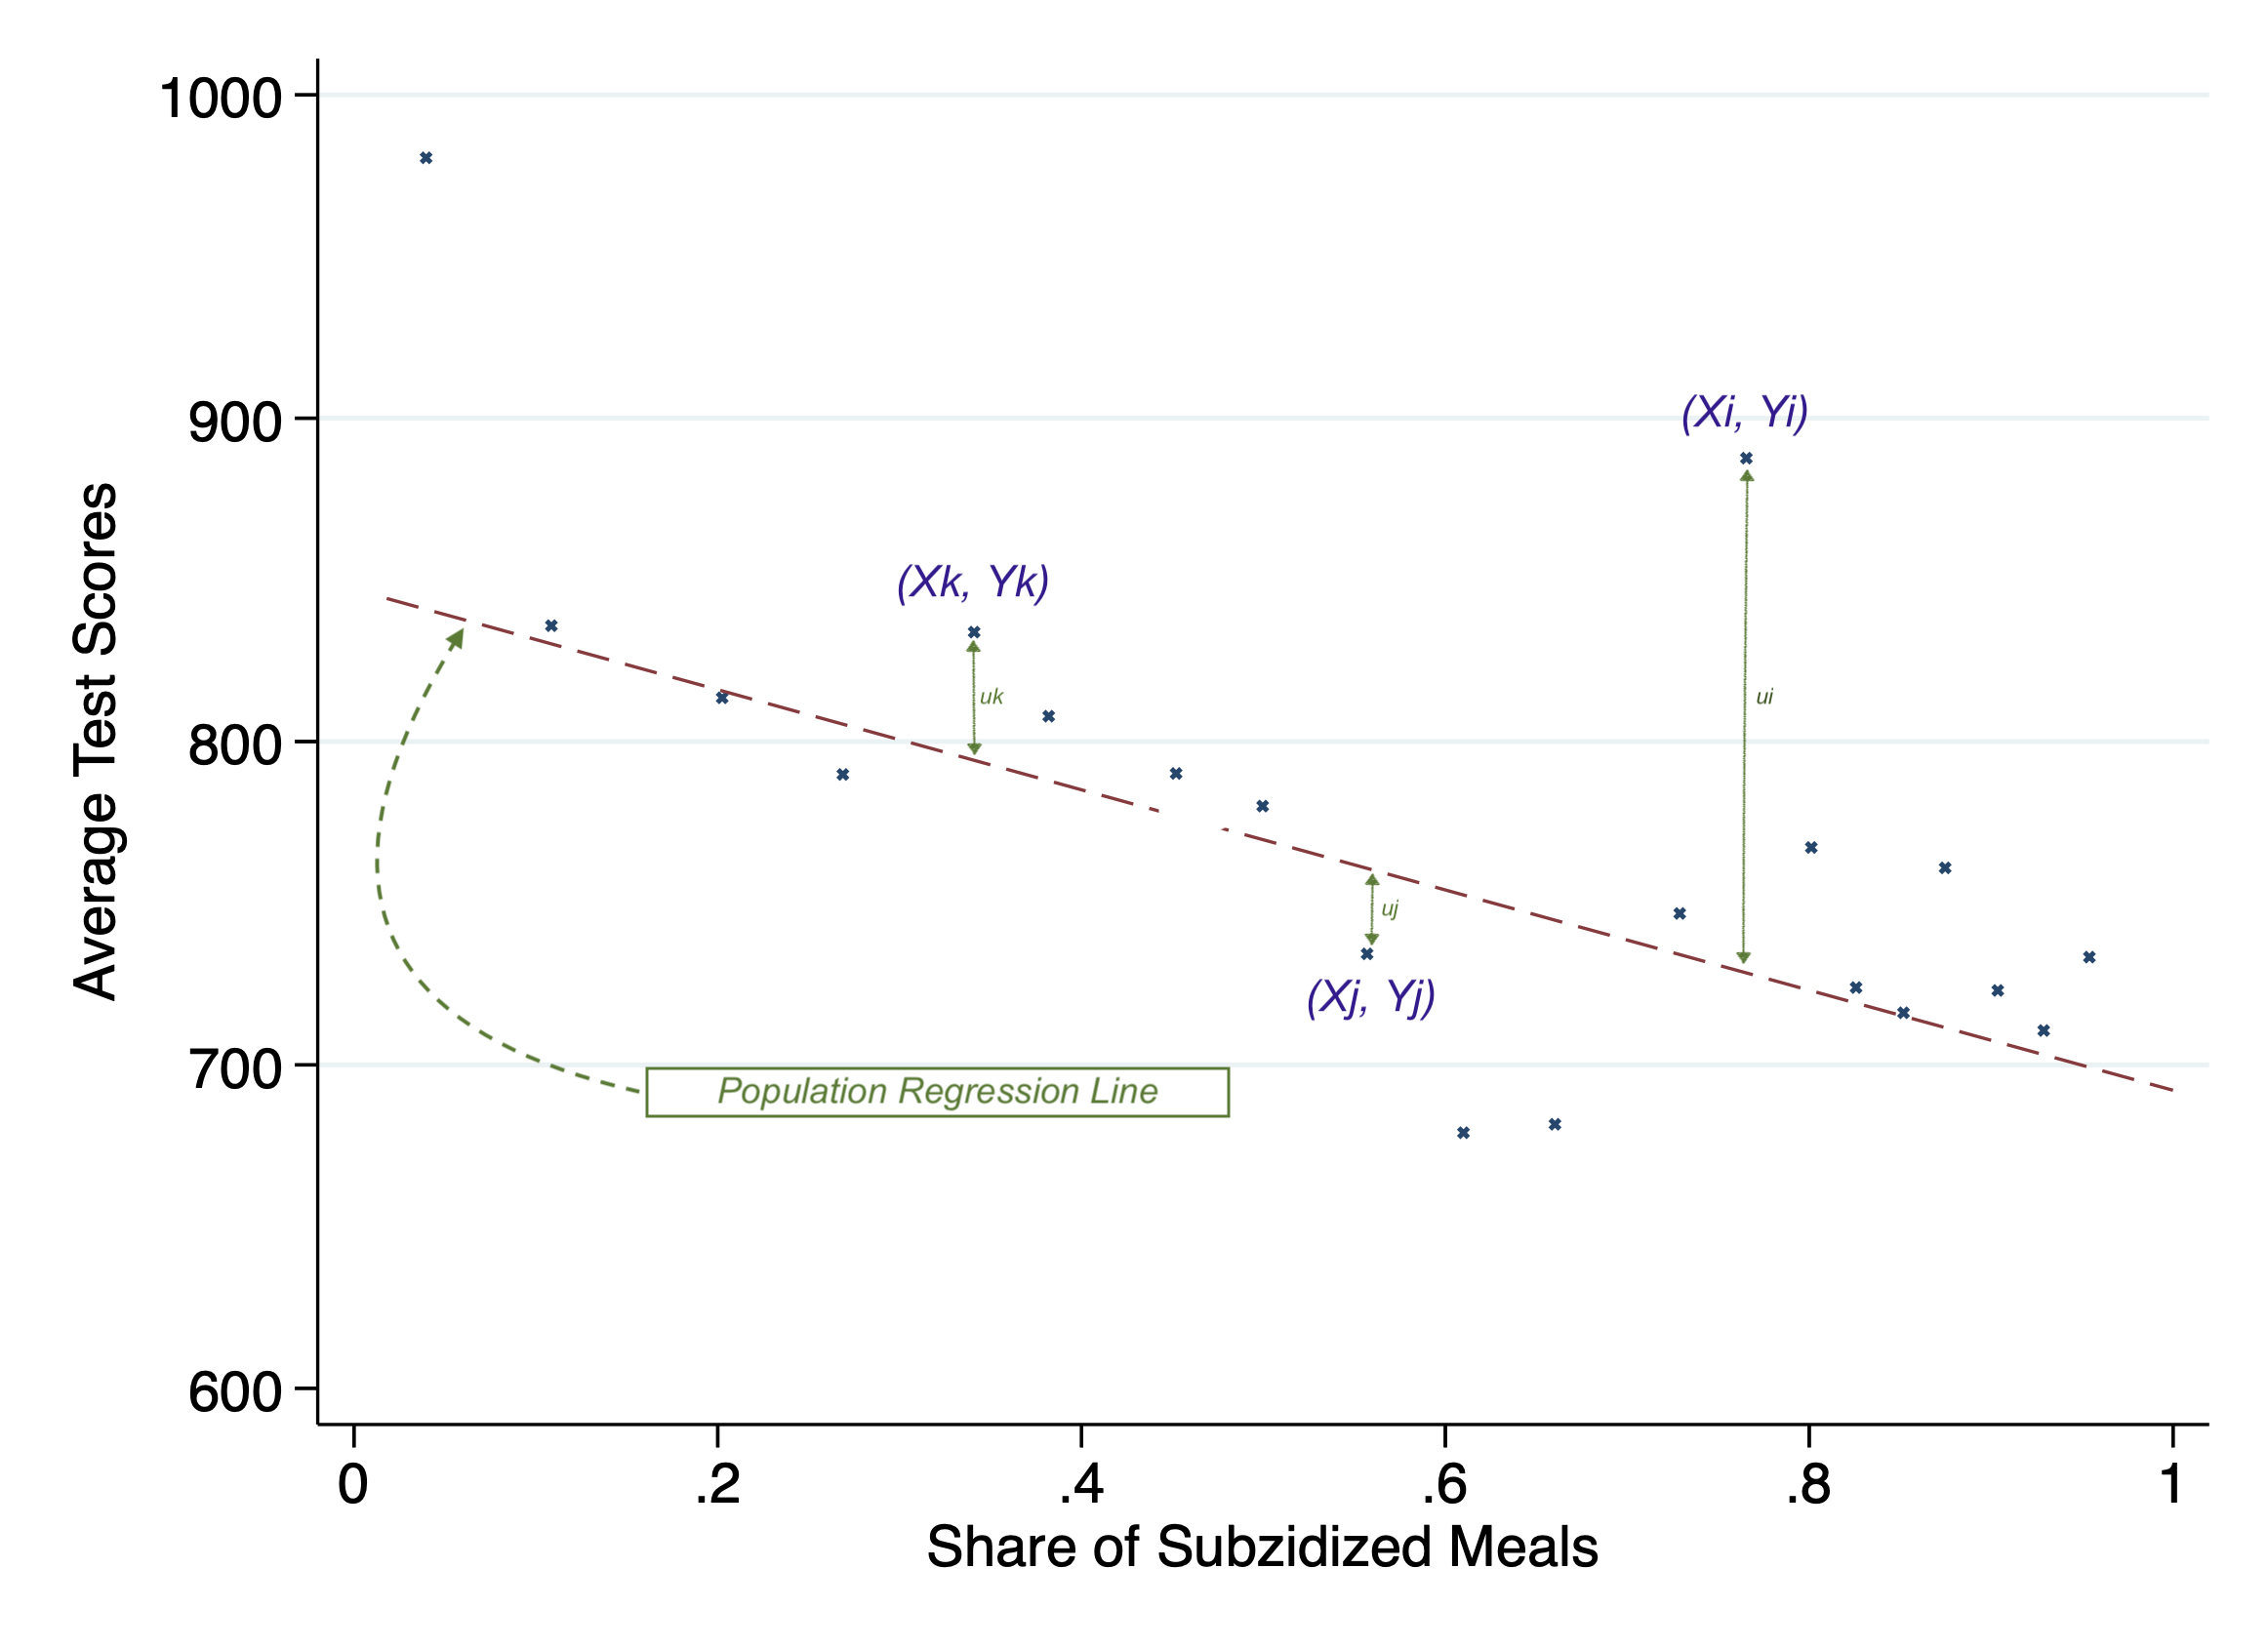
\includegraphics[scale=.25]{images/regression0.png}
\end{figure}
\end{column}
\end{columns}
\end{frame}


\begin{frame}{Interpretation}
Here, the population regression line is given by
\begin{eqnarray*}
     \hat{\beta}_0 \approx 754+155\times.6 \approx 847\\
     \hat{\beta}_1 \approx \frac{ -11.78}{.28^2} \approx -155\\
    \hat{Y}_i \approx 847 -155\times X_i
\end{eqnarray*}
\begin{itemize}
    \item This means that a 10ppt increase in the share of subsidized meals is associated with ($\neq$ cause!) a 15.5 decrease in the average test scores. 
    \item To give a standard of comparison, this is about 26\% of the Test scores' standard deviation!
    \item The intercept (taken literally) means that, according to this estimated line, districts with zero meals would have a (predicted) test score of approximately 847...
    \item But this interpretation of the intercept makes no sense -- it extrapolates the line outside the range of the data (see Lect2 for descriptive stats) -- here, the intercept is not economically meaningful.
\end{itemize}
\end{frame}


\begin{frame}{Example: Estimating an OLS Line with 10 Observations}
\tiny
\begin{columns}[T]
\begin{column}{0.68\textwidth}
\begin{center}
\begin{tabular}{c|c|c|r|r|r|r}
$i$ & $X_i$ & $Y_i$ & $X_i-\overline X$ & $(X_i-\overline X)^2$ & $Y_i-\overline Y$ & $(X_i-\overline X)(Y_i-\overline Y)$ \\ \hline
1 & 1 & 10.8 & -4.5 & 20.25 &  2.31 & -10.40 \\
2 & 2 &  9.4 & -3.5 & 12.25 &  0.91 &  -3.19 \\
3 & 3 &  9.9 & -2.5 &  6.25 &  1.41 &  -3.53 \\
4 & 4 &  8.5 & -1.5 &  2.25 &  0.01 &  -0.01 \\
5 & 5 &  8.8 & -0.5 &  0.25 &  0.31 &  -0.16 \\
6 & 6 &  8.0 &  0.5  &  0.25 & -0.49 &  -0.25 \\
7 & 7 &  7.5 &  1.5  &  2.25 & -0.99 &  -1.49 \\
8 & 8 &  7.9 &  2.5  &  6.25 & -0.59 &  -1.47 \\
9 & 9 &  6.8 &  3.5  & 12.25 & -1.69 &  -5.92 \\
10 & 10 & 7.3 & 4.5  & 20.25 & -1.19 &  -5.36 \\ \hline
\multicolumn{1}{r|}{Sums:} & 55 & 84.90 & 0 & 82.50 & 0 & -31.75
\end{tabular}
\end{center}
\end{column}
\begin{column}{0.30\textwidth}
\begin{center}
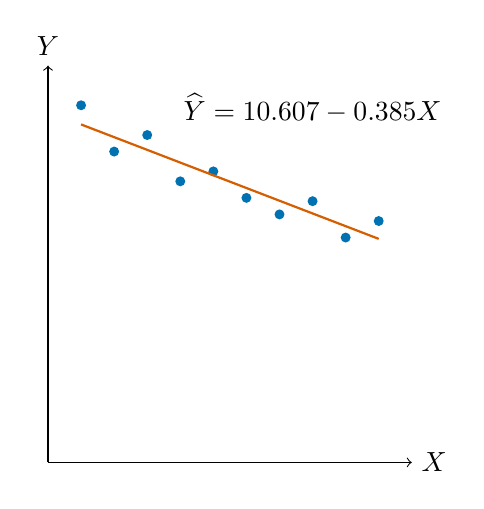
\begin{tikzpicture}[x=.42cm,y=.42cm]
    \draw[->] (0,0) -- (11,0) node[right] {$X$};
    \draw[->] (0,0) -- (0,12) node[above] {$Y$};
    \foreach \x/\y in {
        1/10.8,2/9.4,3/9.9,4/8.5,5/8.8,6/8.0,7/7.5,8/7.9,9/6.8,10/7.3}
        {\fill[blue] (\x,\y) circle (1.8pt);}
    \draw[red,thick] (1,10.22) -- (10,6.76);
    \node[black,anchor=west,fill=white,inner sep=1pt] at (4.0,10.7) {$\widehat{Y}=10.607-0.385X$};
\end{tikzpicture}
\end{center}
\end{column}
\end{columns}
\vspace{-.15cm}
\begin{block}{Calculation}
\scriptsize
\[
\begin{gathered}
\overline{X}=5.5,\quad \overline{Y}=8.49,\\[-2pt]
s_{XY}=\frac{-31.75}{9}=-3.528,\quad
s_X^2=\frac{82.50}{9}=9.167,\\[-2pt]
\hat{\beta}_1=\frac{s_{XY}}{s_X^2}=-0.385,\quad
\hat{\beta}_0=\overline{Y}-\hat{\beta}_1\overline{X}=10.607.
\end{gathered}
\]
\end{block}
\end{frame}

\begin{frame}{Goodness of Fit}
\begin{itemize}
\item How well does our regression model fit the data? This is a crucial question.
\item Goodness of fit measures help us assess the quality of our model.
\item Two regression statistics provide complementary measures of how well the regression line “fits” or explains the data:
\begin{enumerate}
    \item The regression $R^2$ measures the fraction of the variance of Y that is explained by X; it is unitless and ranges between zero (no fit) and one (perfect fit)
    \item The standard error of the regression ($SER$) measures the magnitude of a typical regression residual in the units of Y.
\end{enumerate}
\item These measures are very useful to predict $Y$ when $X$ is known but $Y$ is not (out-of-sample prediction). A common prediction measure is $\hat{Y}\pm SER$.
\end{itemize}
\end{frame}


\begin{frame}{$R^2$}
From the previous slides, we note that
\begin{equation*}
    Y_i = \hat{Y}_i + \hat{U}_i
\end{equation*}
The $R^2$ is the ratio of the sample variance of $\hat{Y}$ to the sample variance of $Y$
\begin{eqnarray*}
    &R^2 &= \frac{\text{explained sum of squares ($ESS$)}}{\text{total sum of squares ($TSS$)}} = \frac{\sum_{i=1}^n (\hat{Y}_i - \overline{Y})^2}{\sum_{i=1}^n (Y_i - \overline{Y})^2}\\
    & &= 1-\frac{\text{sum of squared residuals ($SSR$)}}{\text{total sum of squares ($TSS$)}} = 1-\frac{\sum_{i=1}^n \hat{U}_i^2}{\sum_{i=1}^n (Y_i - \overline{Y})^2}
\end{eqnarray*}
$R^2$ ranges from 0 to 1, where higher values indicate a better fit (i.e., the regressor is good at predicting the outcome)
\end{frame}



\begin{frame}{The Standard Error of the Regression ($SER$)}
\footnotesize
\setlength{\abovedisplayskip}{3pt}
\setlength{\belowdisplayskip}{3pt}
\setlength{\abovedisplayshortskip}{2pt}
\setlength{\belowdisplayshortskip}{2pt}
\textbf{1. Population errors:}
\[
    U_i=Y_i-(\beta_0+\beta_1X_i).
\]
If $\mathbb{E}[U_i]=0$, then
\[
    \sigma_U^2=\operatorname{Var}(U_i)=\mathbb{E}[U_i^2],\text{ and }
    \sigma_U=\sqrt{\mathbb{E}[U_i^2]}.
\]
$\sigma_U$ measures the typical spread around the population regression line, in units of $Y$.
\par\medskip
\textbf{2. Observable residuals:} The true coefficients are unknown, so replace them by their estimates:
\[
    \hat{U}_i=Y_i-(\hat{\beta}_0+\hat{\beta}_1X_i).
\]
The intercept first-order condition gives
\[
    -2\sum_{i=1}^n\hat{U}_i=0,\text{ hence }\overline{\hat{U}}=0.
\]
\par\medskip
\textbf{3. Estimate the error variance and standard deviation:}
\[
    \hat{\sigma}_U^2=\frac{1}{n-2}\sum_{i=1}^n(\hat{U}_i-\overline{\hat{U}})^2
    =\frac{SSR}{n-2};
    \text{ and }SER=\hat{\sigma}_U=\sqrt{\hat{\sigma}_U^2}.
\]
The $n-2$ denominator corrects for estimating the intercept and slope.
\par\medskip
Under the usual homoskedastic OLS assumptions, $SER^2$ is unbiased for $\sigma_U^2$; $SER$ estimates $\sigma_U$.
\par\smallskip
As with the sample standard deviation $s_Y$, we estimate an unknown spread from deviations around a fitted mean; see the comparison next.
\end{frame}

\begin{frame}{From the Sample Standard Deviation to SER}
\footnotesize
\setlength{\abovedisplayskip}{4pt}
\setlength{\belowdisplayskip}{4pt}
\begin{columns}[T,onlytextwidth]
\begin{column}{0.48\textwidth}
\textbf{Before: unknown $\sigma_Y$}
\par\smallskip
We want to estimate the population variance:
\[
\sigma_Y^2=\mathbb{E}\big[(Y_i-\mu_Y)^2\big].
\]
Estimate the mean $\mu_Y$ by $\overline Y$: \textbf{one fitted parameter}, hence $n-1$.
\[
s_Y^2=\frac{\sum_{i=1}^n(Y_i-\overline Y)^2}{n-1},
\qquad s_Y=\sqrt{s_Y^2}.
\]
$s_Y$ estimates the outcome spread $\sigma_Y$.
\end{column}
\begin{column}{0.48\textwidth}
\textbf{Regression: unknown $\sigma_U$}
\par\smallskip
We want to estimate the error variance:
\[
\sigma_U^2=\mathbb{E}[U_i^2],\text{ since }\mathbb{E}[U_i]=0.
\]
Estimate the mean $\beta_0+\beta_1X_i$ by $\hat Y_i$: \textbf{two fitted parameters}, hence $n-2$.
\[
\hat U_i=Y_i-\hat Y_i,\text{ and }
SER^2=\frac{\sum_{i=1}^n\hat U_i^2}{n-2}.
\]
$SER=\sqrt{SER^2}$ estimates the error spread $\sigma_U$.
\end{column}
\end{columns}
\par\medskip
\textbf{The comparison:} $s_Y$ estimates the spread of outcomes around $\mu_Y$; $SER$ estimates the spread of regression errors around the regression line.
\end{frame}


\begin{frame}{SER and RMSE: What Is the Difference?}
\footnotesize
Both measures summarize the typical size of the OLS residuals.
\begin{itemize}
    \item First define the residual sum of squares:
    \[
        SSR=\sum_{i=1}^n \hat{U}_i^2.
    \]
    \item The $SER$ divides by $n-2$:
    \[
        SER=\sqrt{\frac{SSR}{n-2}}.
    \]
    The two degrees of freedom are used to estimate $\beta_0$ and $\beta_1$.
    \item The fitted value is $\widehat{Y}_i=\widehat{\beta}_0+\widehat{\beta}_1X_i$, so the prediction error is
    \[
        Y_i-\widehat{Y}_i=\widehat{U}_i.
    \]
    Therefore, the $RMSE$ is the root mean squared prediction error:
    \[
        RMSE=\sqrt{\frac{SSR}{n}}.
    \]
    It is the average size of the errors $Y_i-\widehat{Y}_i$ in the observed sample.
    \item For a large $n$, $n-2$ and $n$ are almost the same, so $SER$ and $RMSE$ are very similar.
\end{itemize}
\begin{block}{Interpretation}
Both are measured in the units of $Y$. They describe the typical size of the part of $Y$ that the regression does not explain.
\end{block}
\end{frame}


\begin{frame}{Goodness of Fit}
 \begin{columns}
\begin{column}{0.35\textwidth}
\begin{itemize}
    \item Here the $R^2=.509$ and $RMSE=42.601$
    \item About half of the variation in actual test scores is explained by the variation in the predicted test scores (which, in our regression specification, comes from the variation in subsidized meals).
    \item Does this make sense? Does this mean that subsidizing school meals matters for education in a policy sense?
\end{itemize}
\end{column}
\begin{column}{0.7\textwidth}
\begin{figure}
  \centering
         \vspace{-1mm}
        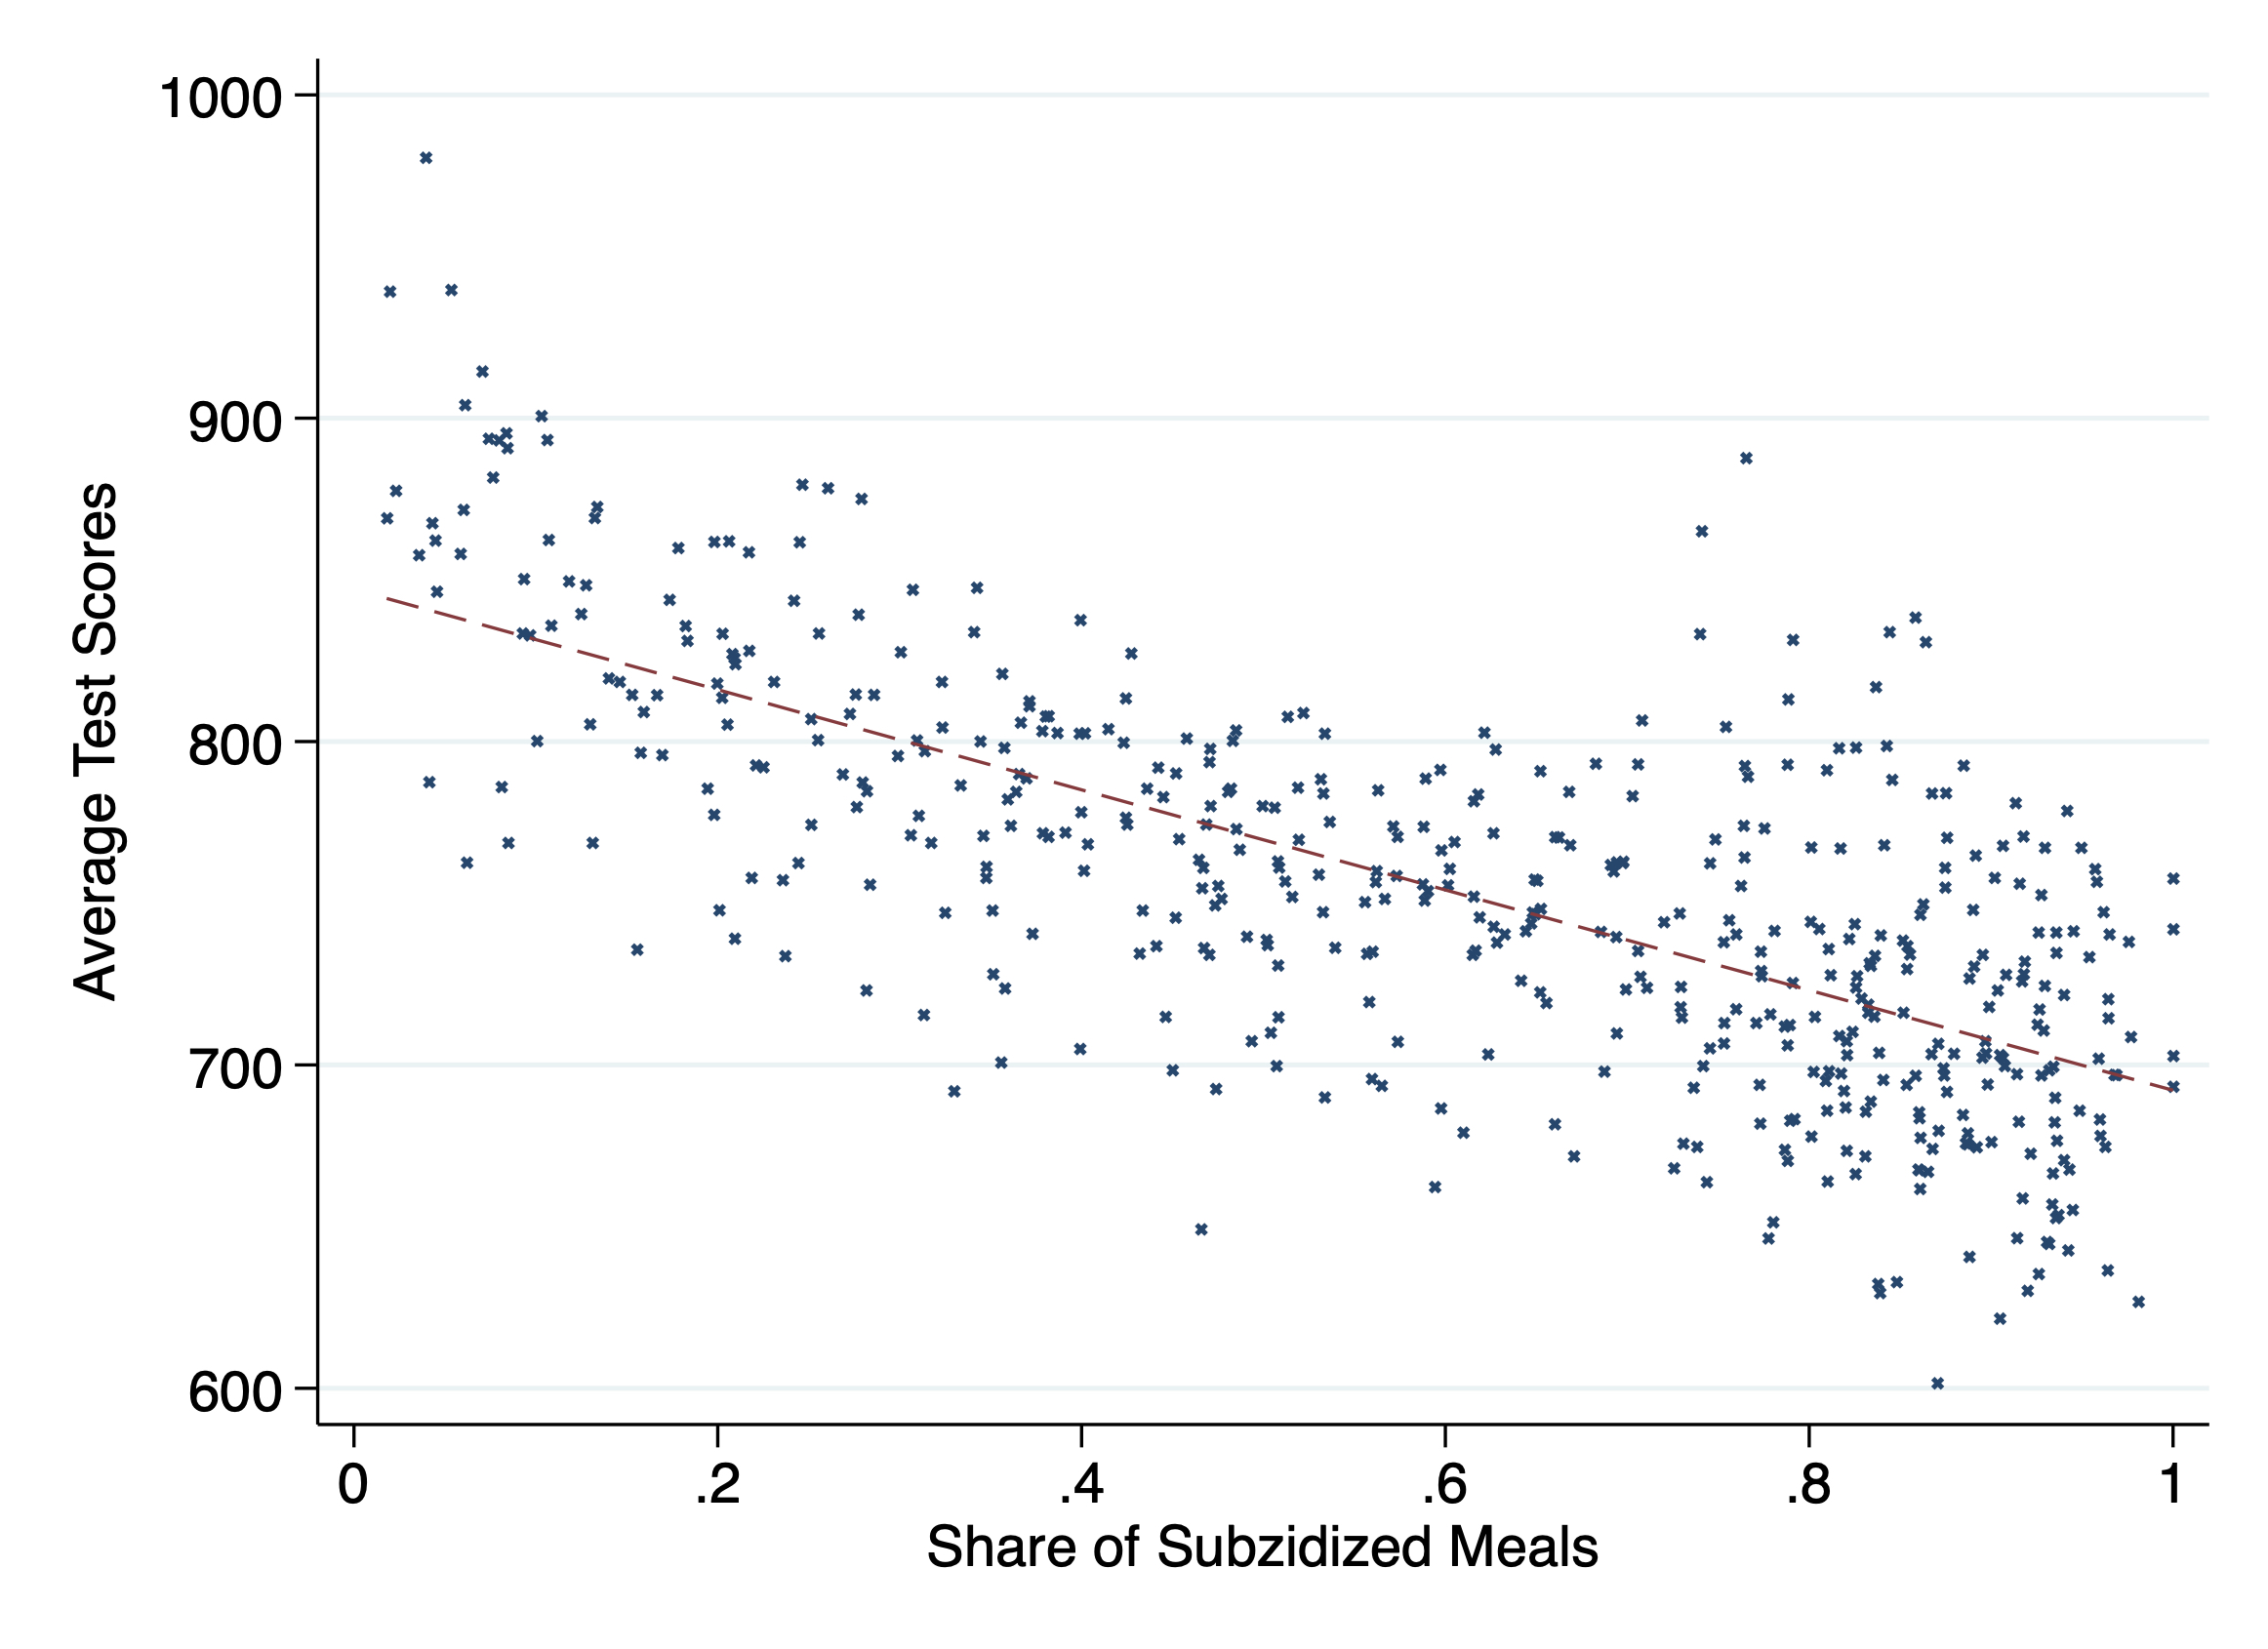
\includegraphics[scale=.25]{images/testscores_corr.png}
\end{figure}
\end{column}
\end{columns}
\end{frame}


\begin{frame}{Population OLS: FOCs and Results}
In the population, choose $(\hat{\beta}_0,\hat{\beta}_1)$ to minimize the mean squared prediction error:
\[
Q(\hat{\beta}_0,\hat{\beta}_1)=\mathbb{E}\left[(Y-\hat{\beta}_0-\hat{\beta}_1X)^2\right].
\]
The population first-order conditions are
\begin{align*}
0=\frac{\partial Q}{\partial \hat{\beta}_0}
  &=-2\mathbb{E}[Y-\hat{\beta}_0-\hat{\beta}_1X],\\
0=\frac{\partial Q}{\partial \hat{\beta}_1}
  &=-2\mathbb{E}[X(Y-\hat{\beta}_0-\hat{\beta}_1X)].
\end{align*}
The first condition gives
\[
    \hat{\beta}_0=\mathbb{E}[Y]-\hat{\beta}_1\mathbb{E}[X].
\]
Substituting this into the second condition gives the population OLS coefficients:
\[
    \hat{\beta}_1=\frac{\operatorname{Cov}(X,Y)}{\operatorname{Var}(X)},
    \qquad
    \hat{\beta}_0=\mathbb{E}[Y]-\hat{\beta}_1\mathbb{E}[X].
\]
\end{frame}


\begin{frame}{The conditions for causality}
\begin{exampleblock}{The OLS Assumptions for Causal Inference}
Let
    \begin{equation*}
        Y_i  =  \beta_0 + \beta_1 X_i + U_i \text{~~;~~} i=1,...,n
    \end{equation*}
where $\beta_1$ is the causal effect of $X$ on $Y$. Then:
    \begin{enumerate}
        \item The error term $U_i$ has conditional mean $0$ given $X_i$: $\mathbb{E}[U_i\mid X_i]=0$;
        \item $(X_i, Y_i)$ $i=1,...,n$, are independent and identically distributed (i.i.d.) draws from their joint distribution; and
        \item Large outliers are unlikely: $X_i$ and $Y_i$ have nonzero finite fourth moments.
    \end{enumerate}
    
\end{exampleblock}
\end{frame}



\begin{frame}{The conditions for causality}
Why do these conditions help us estimate a causal effect?
\begin{enumerate}
    \item \textbf{Causal interpretation:} $\mathbb{E}[U_i\mid X_i]=0$ means that, once $X_i$ is fixed, the remaining determinants of $Y_i$ in $U_i$ are not systematically related to $X_i$. Therefore, the variation in $Y$ associated with $X$ identifies $\beta_1$ rather than a confounding factor.
    \item \textbf{Reliable estimation:} i.i.d. sampling makes the observations representative of the population and prevents dependence across observations from distorting the OLS calculation.
    \item \textbf{Reliable inference:} finite moments and no large outliers ensure that no single observation dominates the estimate and allow the usual large-sample results for standard errors, tests, and confidence intervals.
\end{enumerate}
\textit{Do you think these assumptions hold in our California Schools Experiment?}
\end{frame}



\begin{frame}{Do the assumptions hold in the California Schools Experiment?}
\footnotesize
\begin{enumerate}
    \item \textbf{Conditional mean zero: likely questionable.} Let $Z_i$ measure students' economic disadvantage and suppose
    \[
        Y_i=\beta_0+\beta_1X_i+\gamma Z_i+V_i,
        \text{ and }\mathbb{E}[Z_i\mid X_i=1]\neq\mathbb{E}[Z_i\mid X_i=0].
    \]
    The regression we estimate omits $Z_i$ and writes
    \[
        Y_i=\beta_0+\beta_1X_i+U_i.
    \]
    Comparing this equation with the true equation above,
    \[
        \beta_0+\beta_1X_i+U_i
        =\beta_0+\beta_1X_i+\gamma Z_i+V_i,
    \]
    so, after subtracting $\beta_0+\beta_1X_i$ from both sides,
    \begin{align*}
        U_i&=\gamma Z_i+V_i,\\
        \mathbb{E}[U_i\mid X_i=x]
        &=\gamma\mathbb{E}[Z_i\mid X_i=x]+\mathbb{E}[V_i\mid X_i=x].
    \end{align*}
    If $\mathbb{E}[V_i\mid X_i=x]=0$, then
    \[
    \mathbb{E}[U_i\mid X_i=1]-\mathbb{E}[U_i\mid X_i=0]
    =\gamma\left[\mathbb{E}[Z_i\mid X_i=1]-\mathbb{E}[Z_i\mid X_i=0]\right]\neq 0.
    \]
    Thus, the zero conditional-mean assumption fails.
    \item \textbf{i.i.d. sampling: plausible with care.} If schools are sampled randomly from the same population, the observations can be treated as i.i.d. draws. If schools are clustered by district or selected through a non-random process, this assumption needs more justification.
    \item \textbf{No influential outliers: must be checked.} A school with an unusually large test score or subsidized-meal rate could strongly affect the fitted line and the estimated effect.
\end{enumerate}
The main threat to a causal interpretation is the first assumption: differences between schools may be correlated with both meal subsidies and test scores.
\end{frame}


\begin{frame}{Assumption (1) : $\mathbb{E}[U_i\mid X_i]=0$}
 \begin{columns}
\begin{column}{0.35\textwidth}
\begin{itemize}
\item If \(\mathbb{E}[U_i\mid X_i] \neq 0\), it implies that there is systematic variation in \(Y\) not explained by \(X\).
\item This unexplained variation can confound our causal interpretations, making it challenging to isolate the true causal effect of \(X\) on \(Y\).
\end{itemize}
\end{column}
\begin{column}{0.7\textwidth}
\begin{figure}
  \centering
         \vspace{-1mm}
        \resizebox{!}{0.70\textheight}{% Conditional outcome distributions, with the lecture's expectation notation.
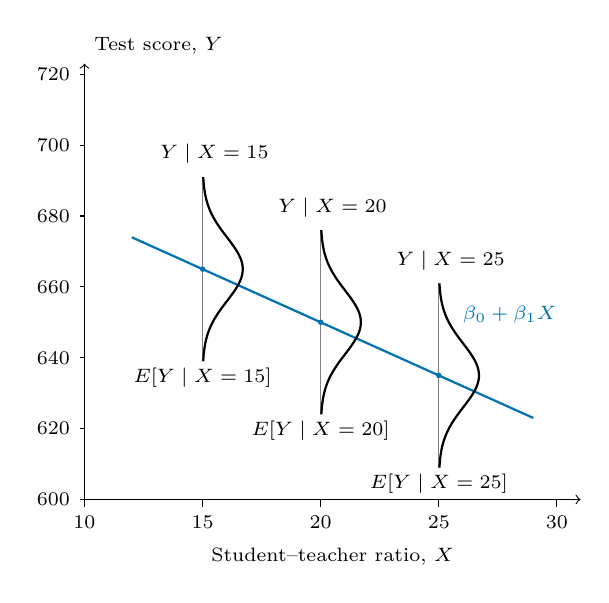
\begin{tikzpicture}[x=0.30cm,y=0.045cm,font=\scriptsize]
\draw[->] (10,600)--(31,600);
\node[below] at (20.5,589) {Student--teacher ratio, $X$};
\draw[->] (10,600)--(10,723) node[above right]{Test score, $Y$};
\foreach \x in {10,15,20,25,30}
  \draw (\x,600)--(\x,598) node[below]{\x};
\foreach \y in {600,620,640,660,680,700,720}
  \draw (10,\y)--(9.8,\y) node[left]{\y};
\draw[blue,thick] (12,674)--(29,623);
\foreach \x/\m in {15/665,20/650,25/635}{
  \draw[gray] (\x,\m-26)--(\x,\m+26);
  \draw[thick,domain=-26:26,samples=65,variable=\t]
    plot ({\x+1.7*exp(-\t*\t/162)},{\m+\t});
  \fill[blue] (\x,\m) circle (1pt);
  \node[above,align=center] at (\x+0.5,\m+27)
    {$Y\mid X=\x$};
  \node[below,fill=white,inner sep=1pt] at (\x,\m-27)
    {$\mathbb{E}[Y\mid X=\x]$};
}
\node[above,blue] at (28,647) {$\beta_0+\beta_1X$};
\end{tikzpicture}
}
\end{figure}
\end{column}
\end{columns}
\end{frame}



\begin{frame}{Assumption (1) : $\mathbb{E}[U_i\mid X_i]=0$}
Then
\begin{eqnarray*}
    & \hat{\beta}_1 &= \frac{cov(X,[\beta_0 + \beta_1 X + U])}{var(X)}\\
    & &= \frac{cov(X,\beta_0)}{var(X)}+\frac{cov(X,\beta_1 X)}{var(X)}+\frac{cov(X,U)}{var(X)}\\
    & &= \beta_1+\frac{cov(X,U)}{var(X)}
\end{eqnarray*}
If $\mathbb{E}[U_i\mid X_i]\neq 0$, then $cov(X,U) \neq 0$... In the California Schools Experiment, schools subsidizing meals (vs. not) are likely to welcome students from poor (vs. rich) economic and social backgrounds -- biasing estimates downwards!
\end{frame}



\begin{frame}{Assumption (2): i.i.d. draws}
This arises automatically if the entity (individual, district) is sampled by simple random sampling:
\begin{itemize}
    \item The entities are selected from the same population, so $(X_i, Y_i)$  are identically distributed for all $i=1,...,n$.
    \item The entities are selected at random, so the values of $(X, Y)$ for different entities are independently distributed.
\end{itemize}
The main place we will encounter non-i.i.d. sampling is when data are recorded over time for the same entity (panel data and time series data) – we will deal with that complication when we cover panel data.
\end{frame}



\begin{frame}{Assumption (3): No large outliers}
 \begin{columns}
\begin{column}{0.35\textwidth}
\begin{itemize}
\item If $X$ and $Y$ are bounded, then they have finite fourth moments. (Standardized test scores automatically satisfy this; family income, etc. satisfy this too.)
\item The substance of this assumption is that a large outlier can strongly influence the results
\item Why is it an outlier? Is it a typo? In practice, outliers are often data glitches (coding or recording problems). If so, they really shouldn’t be in your data set!
\end{itemize}
\end{column}
\begin{column}{0.7\textwidth}
\begin{figure}
  \centering
         \vspace{-1mm}
        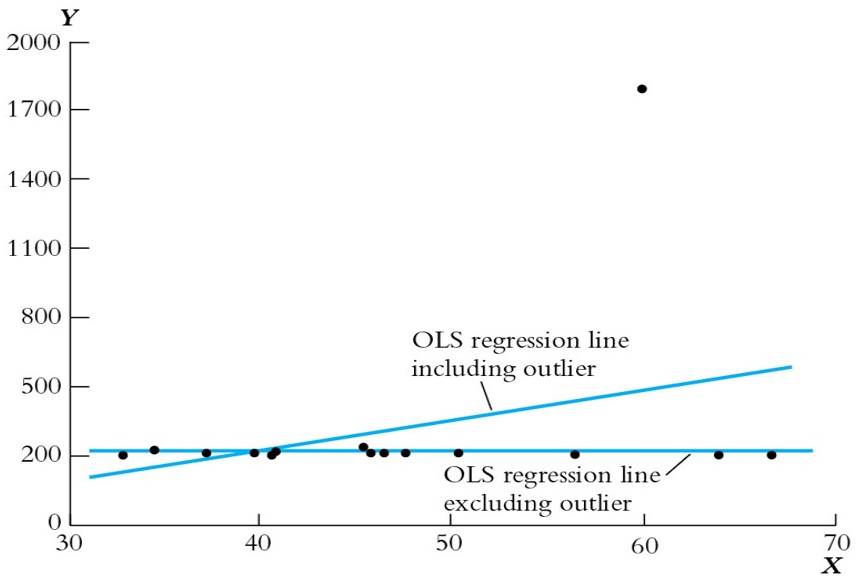
\includegraphics[scale=.6]{images/ols_assumption_2.png}
\end{figure}
\end{column}
\end{columns}
\end{frame}


\begin{frame}{A conditional-expectation rule}
When conditioning on $X$, any function of $X$ is already known:
\[
    \mathbb{E}[XY\mid X]=X\,\mathbb{E}[Y\mid X].
\]
Fix $X=x$. Then $x$ is a constant inside the conditional expectation:
\[
    \mathbb{E}[XY\mid X=x]=\mathbb{E}[xY\mid X=x]
    =x\,\mathbb{E}[Y\mid X=x].
\]
Because this holds for every possible value $x$, we can write the result using the random variable $X$.
\end{frame}


\begin{frame}{OLS Finite Sample Properties}
\footnotesize
\setlength{\abovedisplayskip}{3pt}
\setlength{\belowdisplayskip}{3pt}
Start from the OLS slope formula and substitute
$Y_i=\beta_0+\beta_1X_i+U_i$, using $\sum_i(X_i-\overline X)=0$:
\[
\hat{\beta}_1
=\frac{\sum_i(X_i-\overline X)(Y_i-\overline Y)}{\sum_i(X_i-\overline X)^2}
=\frac{\sum_i(X_i-\overline X)Y_i}{\sum_i(X_i-\overline X)^2}
=\frac{\sum_i(X_i-\overline X)(\beta_0+\beta_1X_i+U_i)}
        {\sum_i(X_i-\overline X)^2}.
\]
Because $\sum_i(X_i-\overline X)=0$, the intercept term disappears. For the
$\beta_1$ term, use $X_i=\overline X+(X_i-\overline X)$:
\[
\sum_i(X_i-\overline X)X_i
=\sum_i(X_i-\overline X)\left[\overline X+(X_i-\overline X)\right]
=\overline X\sum_i(X_i-\overline X)+\sum_i(X_i-\overline X)^2
=\sum_i(X_i-\overline X)^2.
\]
Therefore,
\[
\hat{\beta}_1=\beta_1+
\frac{\sum_{i=1}^n(X_i-\overline X)U_i}
     {\sum_{i=1}^n(X_i-\overline X)^2}.
\]
\textbf{1. Conditional unbiasedness:} hold $X$ fixed and use $\mathbb{E}[U_i\mid X]=0$.
\[
\mathbb{E}[\hat\beta_1\mid X]
=\beta_1+
\frac{\sum_i(X_i-\overline X)\mathbb{E}[U_i\mid X]}
{\sum_i(X_i-\overline X)^2}
=\beta_1+0=\boxed{\beta_1}.
\]
\textbf{2. Unconditional unbiasedness:} apply the law of iterated expectations.
\[
\mathbb{E}[\hat\beta_1]
=\mathbb{E}\!\left[\mathbb{E}[\hat\beta_1\mid X]\right]
=\mathbb{E}[\beta_1]=\boxed{\beta_1}.
\]
\end{frame}

\begin{frame}{OLS Finite Sample Properties}
\scriptsize
\setlength{\abovedisplayskip}{3pt}
\setlength{\belowdisplayskip}{3pt}
\textbf{Reminder: $SER$ estimates $\sigma_U$, so $SER^2$ estimates $\sigma_U^2$.}
\par\smallskip
Write $\hat\beta_1-\beta_1$ as a weighted sum of errors. Conditional on $X$, the weights are fixed; independence makes the variance of the sum equal to the sum of variances. Under homoskedasticity, $var(U_i\mid X)=\sigma_U^2$.
\par\smallskip
Define $TSS_X=\sum_{i=1}^n(X_i-\overline X)^2$, the \textbf{total sum of squares of $X$}: total variation of the observed $X_i$ values around their sample mean.
\[
\begin{aligned}
var(\hat\beta_1\mid X)
&=var(\hat\beta_1-\beta_1\mid X)
=var\left[\frac{\sum_{i=1}^n(X_i-\overline X)U_i}{TSS_X}\Bigg|X\right]\\
&=\frac{1}{TSS_X^2}var\left[\sum_{i=1}^n(X_i-\overline X)U_i\Bigg|X\right]\\
&=\frac{\sum_{i=1}^n(X_i-\overline X)^2var(U_i\mid X)}{TSS_X^2}
=\frac{\sigma_U^2\sum_{i=1}^n(X_i-\overline X)^2}{TSS_X^2}
=\frac{\sigma_U^2}{TSS_X}.
\end{aligned}
\]
\textbf{Plug in the estimated error variance:}
\[
\widehat{\operatorname{Var}}(\hat\beta_1\mid X)
=\frac{SER^2}{TSS_X}
=\frac{SSR}{(n-2)TSS_X};
\qquad
\widehat{SE}(\hat\beta_1)=\frac{SER}{\sqrt{TSS_X}}.
\]
\textbf{Connection to the sample mean:} $TSS_X=(n-1)s_X^2$, so it grows approximately in proportion to $n$ when the spread of $X$ stays similar.
\[
\widehat{SE}(\hat\beta_1)=\frac{SER}{s_X\sqrt{n-1}},
\text{ compared with }\widehat{SE}(\overline Y)=\frac{s_Y}{\sqrt n}.
\]
With similar regressor spread and error variance, the slope's standard error also decreases roughly as $1/\sqrt n$: quadrupling $n$ approximately halves it.
\end{frame}

% \begin{frame}{OLS Sample Properties --- $\mathbb{E}[\hat{\beta}_0]=\beta_0$}
% %Note that
% \begin{eqnarray*}
% &\mathbb{E}[\hat{\beta}_0] &=\mathbb{E}[\overline{Y}_i-\hat{\beta}_1\overline{X}] \\
% & &=\mathbb{E}[\beta_0 + \beta_1 \overline{X} + \frac{1}{n}\sum_{i=1}^n U_i -\hat{\beta}_1\overline{X}] \\
% & &=\beta_0 + \mathbb{E}[\beta_1 -\hat{\beta}_1] \overline{X} + \frac{1}{n}\sum_{i=1}^n \mathbb{E}[U_i]\\
% & &=\beta_0 + \frac{1}{n}\sum_{i=1}^n \mathbb{E}[\mathbb{E}[U_i\mid X]]\\
% & &=\beta_0 
% \end{eqnarray*}
% \end{frame}


\begin{frame}{OLS Finite Sample Properties}
\footnotesize
\setlength{\abovedisplayskip}{4pt}
\setlength{\belowdisplayskip}{4pt}
 \begin{columns}
\begin{column}{0.52\textwidth}
\begin{itemize}
    \item \textbf{Hold the observed $X$ values fixed.} Under homoskedasticity,
    \[
    \operatorname{Var}(\hat\beta_1\mid X)=\frac{\sigma_U^2}{TSS_X}.
    \]
    \item Estimate the unknown $\sigma_U^2$ by $SER^2=SSR/(n-2)$:
    \[
    \widehat{\operatorname{Var}}(\hat\beta_1\mid X)
    =\frac{SER^2}{TSS_X}
    =\frac{SSR}{(n-2)TSS_X}.
    \]
    \item Larger error variance increases the slope's conditional variance: there is more noise around the regression line.
\end{itemize}
\end{column}
\begin{column}{0.46\textwidth}
\begin{figure}
  \centering
         \vspace{-1mm}
        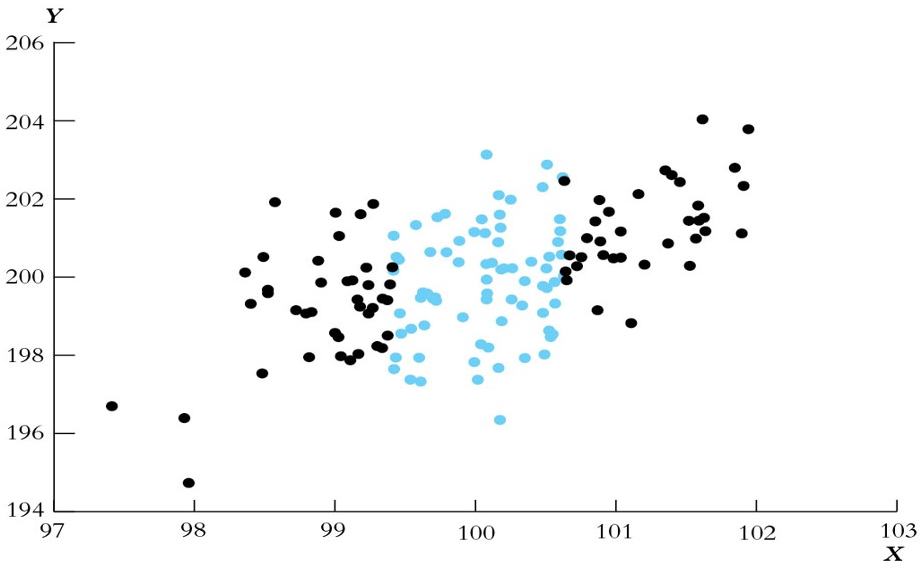
\includegraphics[width=\linewidth]{images/variance_x.png}
\end{figure}
\end{column}
\end{columns}
\begin{itemize}
    \item Holding error variance fixed, more variation in the observed $X$ values increases $TSS_X$ and reduces $\operatorname{Var}(\hat\beta_1\mid X)$.
    \item With similar regressor spread and error variance, a larger sample increases $TSS_X$ and reduces the slope's conditional variance.
    \item Ideally, we would choose $X$ to be as spread out as possible -- this is sometimes possible with experimental data, but in practice, we often work with random samples
\end{itemize}
\end{frame}



\begin{frame}{OLS Finite Sample Properties}
\footnotesize
\setlength{\abovedisplayskip}{4pt}
\setlength{\belowdisplayskip}{4pt}
Let $\mathbf{X}=(X_1,\ldots,X_n)$ denote the full regressor sample,
$\bar U=n^{-1}\sum_i U_i$, and $TSS_X=\sum_i(X_i-\bar X)^2>0$.
Assume $\mathbb{E}[U_i\mid\mathbf{X}]=0$ for every $i$.
\begin{enumerate}
\item \textbf{Average the population equation} $Y_i=\beta_0+\beta_1X_i+U_i$:
\[
\bar Y=\beta_0+\beta_1\bar X+\bar U.
\]
\item \textbf{Substitute into the OLS intercept}:
\[
\hat\beta_0=\bar Y-\hat\beta_1\bar X
=\beta_0+\bar U-\bar X(\hat\beta_1-\beta_1).
\]
\item \textbf{Condition on $\mathbf{X}$}, so $\bar X$ is fixed:
\[
\begin{aligned}
\mathbb{E}[\hat\beta_0\mid\mathbf{X}]
&=\beta_0+\mathbb{E}[\bar U\mid\mathbf{X}]
-\bar X\bigl(\mathbb{E}[\hat\beta_1\mid\mathbf{X}]-\beta_1\bigr)\\
&=\beta_0+0-\bar X\cdot0=\beta_0.
\end{aligned}
\]
Here $\mathbb{E}[\bar U\mid\mathbf{X}]=n^{-1}\sum_i\mathbb{E}[U_i\mid\mathbf{X}]=0$;
conditional unbiasedness of the slope was derived earlier.
\end{enumerate}
By the law of iterated expectations,
$\mathbb{E}[\hat\beta_0]=\mathbb{E}[\mathbb{E}[\hat\beta_0\mid\mathbf{X}]]=\beta_0$.
\end{frame}

\begin{frame}{OLS Finite Sample Properties}
\footnotesize
\setlength{\abovedisplayskip}{4pt}
\setlength{\belowdisplayskip}{4pt}
Assume conditionally uncorrelated errors and homoskedasticity:
$\operatorname{Var}(U_i\mid\mathbf{X})=\sigma_U^2$.
Write $d_i=X_i-\bar X$. Substituting the slope decomposition gives
\[
\hat\beta_0-\beta_0
=\bar U-\bar X\frac{\sum_i d_i U_i}{TSS_X}
=\sum_i a_i U_i,
\text{ where }a_i=\frac1n-\frac{\bar X d_i}{TSS_X}.
\]
Conditional on $\mathbf{X}$, the weights $a_i$ are fixed and cross covariances vanish:
\[
\operatorname{Var}(\hat\beta_0\mid\mathbf{X})=\sigma_U^2\sum_i a_i^2.
\]
Expand the squared weights:
\[
\begin{aligned}
\sum_i a_i^2
&=\frac{n}{n^2}
-\frac{2\bar X}{nTSS_X}\underbrace{\sum_i d_i}_{=0}
+\frac{\bar X^2}{TSS_X^2}\underbrace{\sum_i d_i^2}_{=TSS_X}\\
&=\frac1n+\frac{\bar X^2}{TSS_X}.
\end{aligned}
\]
Therefore,
\[
\boxed{\operatorname{Var}(\hat\beta_0\mid\mathbf{X})
=\sigma_U^2\left(\frac1n+\frac{\bar X^2}{TSS_X}\right)
=\frac{\sigma_U^2\sum_i X_i^2}{nTSS_X}},
\]
because $\sum_i X_i^2=TSS_X+n\bar X^2$.
\end{frame}



\begin{frame}{Testing Whether the Intercept or Slope Is Zero}
\footnotesize
\setlength{\abovedisplayskip}{3pt}
\setlength{\belowdisplayskip}{3pt}
\textbf{1. Estimate the regression} $Y_i=\beta_0+\beta_1X_i+U_i$ by OLS.
Use $SER=\sqrt{SSR/(n-2)}$ and $TSS_X=\sum_i(X_i-\bar X)^2$.
\par\smallskip
\begin{columns}[T]
\begin{column}{0.48\textwidth}
\textbf{2. Test the intercept}
\[
H_0:\beta_0=0,\text{ against }H_1:\beta_0\ne0.
\]
\[
SE(\hat\beta_0)=SER\sqrt{\frac1n+\frac{\bar X^2}{TSS_X}}.
\]
\[
t_0^{\mathrm{obs}}=\frac{\hat\beta_0}{SE(\hat\beta_0)}.
\]
Is the population regression line's value at $X=0$ different from zero?
\end{column}
\begin{column}{0.48\textwidth}
\textbf{2. Test the slope}
\[
H_0:\beta_1=0,\text{ against }H_1:\beta_1\ne0.
\]
\[
SE(\hat\beta_1)=\frac{SER}{\sqrt{TSS_X}}.
\]
\[
t_1^{\mathrm{obs}}=\frac{\hat\beta_1}{SE(\hat\beta_1)}.
\]
Is the population regression slope different from zero?
\end{column}
\end{columns}
\par\smallskip
\textbf{3. For each test separately, use the normal approximation.}
Under its null, conditional on $X$, $T_j\approx\mathcal{N}(0,1)$ for large $n$,
using the OLS assumptions and homoskedasticity, for $j=0,1$.
\[
p_j\approx2\bigl[1-\Phi(|t_j^{\mathrm{obs}}|)\bigr].
\]
\textbf{4. Decision at 5\%:} reject that null if $|t_j^{\mathrm{obs}}|>1.96$
(equivalently, $p_j<0.05$); otherwise, do not reject it.
\par\smallskip
These are two separate tests at 5\% each, not a joint test that both coefficients are zero.
\end{frame}



\end{document}

